% Final report: Predicting New-User Engagement on Zindi
% Compile: pdflatex report.tex (twice). Figures are produced by ../notebook/zindi_engagement.ipynb into ../figures/.
\documentclass[11pt,a4paper]{article}
\usepackage[T1]{fontenc}
\usepackage[utf8]{inputenc}
\usepackage{lmodern}
\usepackage{mathptmx}
\usepackage{microtype}
\emergencystretch=2em
\usepackage[margin=2.3cm]{geometry}
\usepackage{graphicx,booktabs,amsmath,array,xcolor,enumitem,float,caption}
\usepackage[colorlinks=true,linkcolor=blue!50!black,urlcolor=blue!50!black,citecolor=blue!50!black]{hyperref}
\graphicspath{{../figures/}}
\setlist{itemsep=2pt,topsep=3pt}
\captionsetup{font=small,labelfont=bf}
\newcommand{\code}[1]{\texttt{#1}}

\title{\textbf{Predicting New-User Engagement on Zindi}\\[4pt]
\large Will a user who just signed up still be active in their second month?}
\author{Zhiran Zhang \and Haolin Yang\\[2pt] \small ML with Python, Final Project}
\date{October 2026}

\begin{document}
\maketitle

\begin{abstract}
\noindent
Most people who sign up on Zindi, Africa's largest data-science competition platform, do not come back in their second month.
We predict, at the end of a user's first month, whether the user will be active in the next month.
The masked data first had to be put in time order and labelled by hand.
We then found that the activity log of the last observed month stops on day 22. With the usual whole-month target (\emph{label A}),
the hold-out cohort's labels therefore mean something different from the training labels.
We fix this by measuring every cohort over days 1--22 of the next month (\emph{label B}) and report both versions.
With forward-chaining cross-validation and a grid search over logistic regression, random forest and gradient boosting,
the selected gradient-boosting model reaches F1 = 0.45 on the hold-out cohort with consistent labels (0.47 with label A),
against 0.36--0.40 for the best rule of thumb. The 20\,\% of users it ranks highest contain 62\,\% of all returners.
\end{abstract}

%=====================================================================
\section{Problem statement}
\label{sec:problem}

\paragraph{Context.} Zindi hosts machine-learning competitions and has about 12\,k new sign-ups over the seven months in this dataset.
Most of them are \emph{one-month tourists}: in a typical monthly cohort only 12--21\,\% of new users come back in their second month.

\paragraph{Task.} For each user who registered in month $m$, predict whether the user does \emph{anything} on Zindi
(views a page, joins a competition, submits, posts) in month $m+1$, using only what is known at the end of month $m$.
This is binary classification with a minority positive class.

\paragraph{Why it matters.}
\begin{itemize}
  \item Acquiring users is expensive. A user who survives month 2 is much more likely to become a long-term competitor, community member and potential hire for Zindi's clients.
  \item Churn happens fast. Zindi has to know \emph{at the end of the first month} who is about to drop out, while there is still time to act.
\end{itemize}

\paragraph{How the model helps.}
\begin{itemize}
  \item \textbf{Lower cost through targeted retention:} send onboarding nudges, beginner competitions or mentoring only to the users who need them, instead of contacting everybody.
  \item \textbf{Prioritisation:} pick out likely-engaged newcomers for community programmes and hackathon invitations.
  \item \textbf{Product insight:} show which first-month behaviours (for example submitting versus browsing) go with retention.
\end{itemize}

%=====================================================================
\section{Data, time axis and target}
\label{sec:data}

\subsection{Loading the data with pandas}
The Zindi New User Engagement Prediction Challenge provides eight relational tables linked by \code{User\_ID} and \code{Competition ID}
(Table~\ref{tab:tables}). All tables are loaded with \code{pandas.read\_csv}. Dates are masked: year and month are recoded
(``months are in chronological order but January is not necessarily month 1''), while day of month and time of day are kept.

\begin{table}[H]\centering\small
\begin{tabular}{lrrl}\toprule
Table & Rows & Columns & Content\\\midrule
Users & 12\,413 & 8 & sign-up date, country, two masked features\\
UserActivity & 317\,292 & 6 & page views and clicks (most of the events)\\
CompetitionParticipation & 8\,385 & 8 & competition enrolments, submission counts\\
Discussion & 1\,439 & 9 & forum posts\\
Comments & 467 & 6 & blog comments\\
Competition & 247 & 20 & competition metadata (e.g. secret code = hackathon)\\\bottomrule
\end{tabular}
\caption{Tables used (Blogs and Jobs are not needed).}\label{tab:tables}
\end{table}

\subsection{Recovering the time axis and choosing the test period}
All users are in masked year 1 and in masked months $\{11, 12, 1, \dots, 5\}$. Users can only be active \emph{after} they register,
so the cross-table of sign-up month against activity month must be upper-triangular in the true order (Figure~\ref{fig:time}).
It is, for the order M11 $\to$ M12 $\to$ M1 $\to$ M2 $\to$ M3 $\to$ M4 $\to$ M5.
The M4 cohort has almost no M5 activity (8 of 1\,382 users): Zindi removed it, because the M4 cohort is the official test set.
We therefore built the labels ourselves for cohorts M11--M3, whose next month is observed.

\begin{figure}[H]\centering
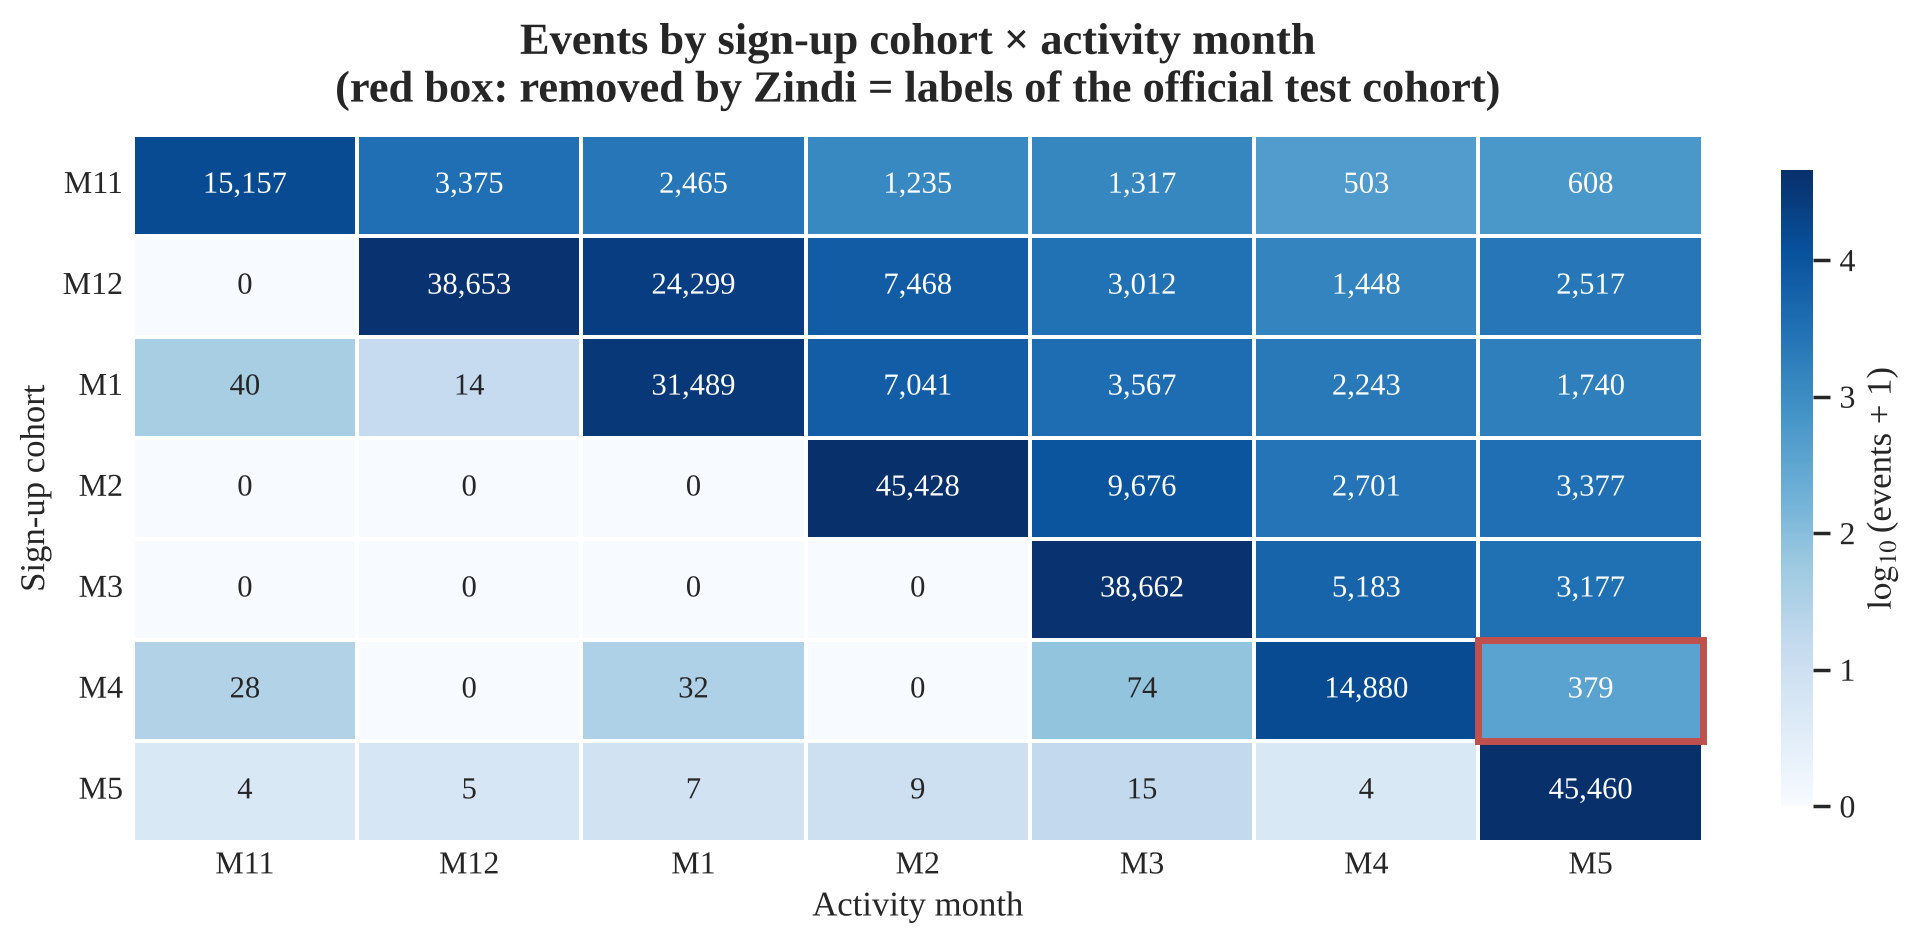
\includegraphics[width=0.78\linewidth]{fig01_time_axis}
\caption{Events by sign-up cohort and activity month. The pattern is upper-triangular, which gives the month order. The red box is the hidden M5 activity of the official test cohort.}
\label{fig:time}
\end{figure}

\paragraph{Test on the latest period.} For time-ordered data the test period must come after the training data,
otherwise the model is trained on the future. The latest labelled cohort, \textbf{M3}, is therefore our hold-out test cohort.
M11--M2 are used for training and cross-validation. Holding out an earlier cohort would either leave a gap in the data or put later cohorts into training.

\subsection{Target definition: two versions of the label}
\label{sec:labels}
\code{Active} = 1 if the user has any record (activity, enrolment, discussion or comment) in the month after sign-up.
Features use only the sign-up month, so the target cannot leak into them.

\paragraph{The problem: truncated hold-out labels.} The label of the hold-out cohort M3 is measured in month M4.
Table~\ref{tab:lastday} shows that the M4 activity log stops on \textbf{day 22}, while enrolments and discussions continue to day 30.
Page views are most of the events, so an M3 user who returns only after day 22 is very likely labelled 0.

\begin{table}[H]\centering\small
\begin{tabular}{lccccccc}\toprule
Last logged day & M11 & M12 & M1 & M2 & M3 & \textbf{M4} & M5\\\midrule
UserActivity & 30 & 31 & 30 & 31 & 31 & \textbf{22} & 27\\
CompetitionParticipation & 30 & 31 & 30 & 31 & 31 & 30 & 27\\
Discussion & 29 & 31 & 30 & 31 & 31 & 30 & 27\\\bottomrule
\end{tabular}
\caption{Last logged day per month and table (month lengths are masked too).}\label{tab:lastday}
\end{table}

With a whole-month label the target does not mean the same thing in training and in testing:
\begin{itemize}
  \item in the training cohorts, $y=1$ means ``active at any point in the next $\sim$30 days'';
  \item in the M3 hold-out, $y=1$ mostly means ``active in the first 22 days of the next month''.
\end{itemize}
The features are aligned (always the sign-up month), but the labels are not. This is a \textbf{label-definition inconsistency}
(measurement inconsistency) between training and evaluation data: the model learns one task and is graded on a slightly different one. It causes
\begin{enumerate}
  \item a \textbf{biased performance estimate} on M3, because a correct prediction for a late returner counts as a false positive;
  \item a \textbf{decision threshold} tuned on cohorts with 17--21\,\% returners being applied to a cohort whose measured rate is pushed down by the truncation;
  \item a \textbf{dip in M3's return rate} that is partly an artefact of the cutoff and could be misread as a real trend.
\end{enumerate}

\paragraph{Our fix.} \textbf{Label B} defines the target as ``active in days 1--22 of the next month'' for \emph{every} cohort, training and test,
so the definitions match. We keep the original whole-month target as \textbf{label A} and run every experiment with both.

Figure~\ref{fig:window} quantifies the issue. In a normal cohort 8--11\,\% of returners are first seen after day 22. In M3 the figure is only 1.6\,\%,
because those late returns are missing from the log. M3 has 243 positives under label A and 239 under label B.

\begin{figure}[H]\centering
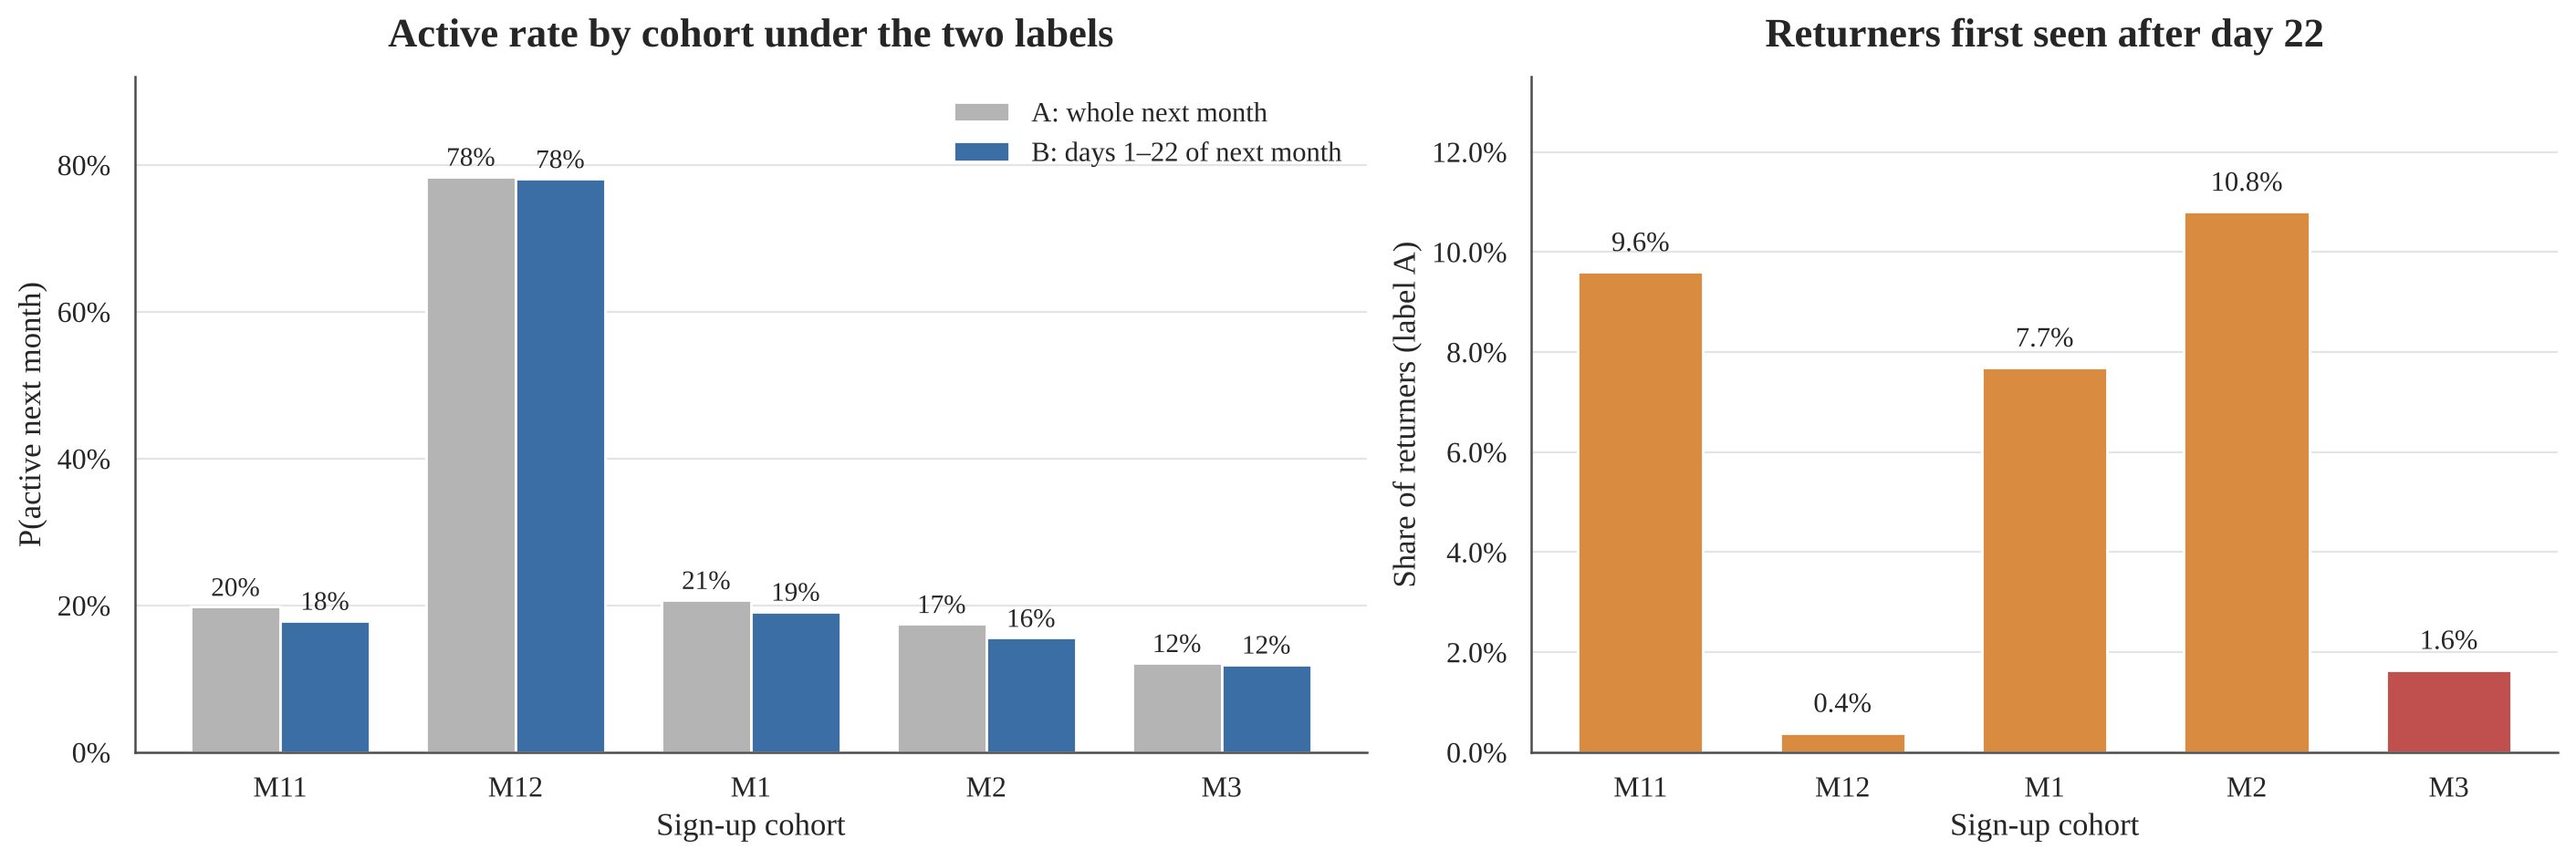
\includegraphics[width=\linewidth]{fig02_label_window}
\caption{Left: active rate per cohort under label A and label B. Right: share of returners whose first next-month record is after day 22; M3 is low because its next month is truncated.}
\label{fig:window}
\end{figure}

\subsection{X / y split}
After feature engineering (Section~\ref{sec:prep}) the labelled cohorts give $X$ with 9\,026 rows and 50 features, and two target vectors
$y_A$ (positive rate 30.5\,\%) and $y_B$ (29.4\,\%). The high overall rate comes from the M12 cohort (Section~\ref{sec:eda}).
The official test set $X_\text{test}$ has the 1\,382 M4 users.

%=====================================================================
\section{Data preparation}
\label{sec:prep}

Table~\ref{tab:prep} lists each transformation and the reason for it.

\begin{table}[H]\centering\small
\begin{tabular}{>{\raggedright}p{4.3cm}>{\raggedright}p{5.2cm}>{\raggedright\arraybackslash}p{5.6cm}}\toprule
Issue & What we do & Why\\\midrule
Events are in long, multi-table logs & aggregate per user, \textbf{sign-up month only} & one row per user; no look-ahead leakage\\
70+ raw event titles (\code{comp\_ID\_xxx}, \dots) & group into 18 behaviour families & IDs are too sparse; the \emph{type} of behaviour generalises\\
\code{Countries\_ID} missing for 47\,\% & category \code{Missing} + binary flag & missingness is informative; imputing would invent data\\
146 masked countries & top 10 kept, rest \code{Other}, one-hot & enough users per level; avoids over-fitting rare countries\\
\code{FeatureY} $\in\{0,1,3\}$ & one-hot & codes are nominal, not ordinal\\
Submission count as strings (\code{"count 10"}) & parse the number; NaN $\to$ 0 & NaN means no successful submission\\
Users with no events in a table & counts $\to$ 0 & absence of activity is a true zero\\
Late sign-ups have less time to act & \code{days\_observed}, \code{active\_day\_ratio}, \code{days\_since\_last} & normalises activity by exposure\\
Masked month lengths; M4 log ends on day 22 & window end = last logged day of the month & exposure features consistent between train and test\\
Target can be measured in two ways & label A (whole month), label B (days 1--22) & label B aligns train and test (Section~\ref{sec:labels})\\\bottomrule
\end{tabular}
\caption{Preparation steps and their motivation.}\label{tab:prep}
\end{table}

\paragraph{Engineered features.}
\begin{itemize}
  \item \textbf{Volume and regularity:} \code{n\_events}, \code{n\_active\_days}, \code{n\_distinct\_actions}, \code{n\_distinct\_comps}, \code{active\_day\_ratio}.
  \item \textbf{Recency:} \code{days\_since\_last}, days between the last activity and the end of the month.
  \item \textbf{Behaviour mix:} counts for the 18 event families (submissions, data downloads, learning pages, jobs, \dots).
  \item \textbf{Competition context:} \code{n\_comps\_joined}, \code{max\_sub\_bucket}, \code{n\_new\_comps\_joined} (competitions first seen in the sign-up month, so likely still running), \code{joined\_hackathon} (competition with a secret code).
  \item \textbf{Community:} \code{n\_discussions}, \code{n\_comments}.
  \item \textbf{Profile:} \code{FeatureX}, \code{FeatureY}, country, \code{country\_missing}, \code{signup\_day}, \code{signup\_hour}, \code{days\_observed}.
\end{itemize}

%=====================================================================
\section{Exploratory analysis}
\label{sec:eda}
The figures use label A; the patterns are the same under label B. Each finding is followed by what it changes in the ML setup.

\subsection{Retention differs strongly by cohort}
\begin{figure}[H]\centering
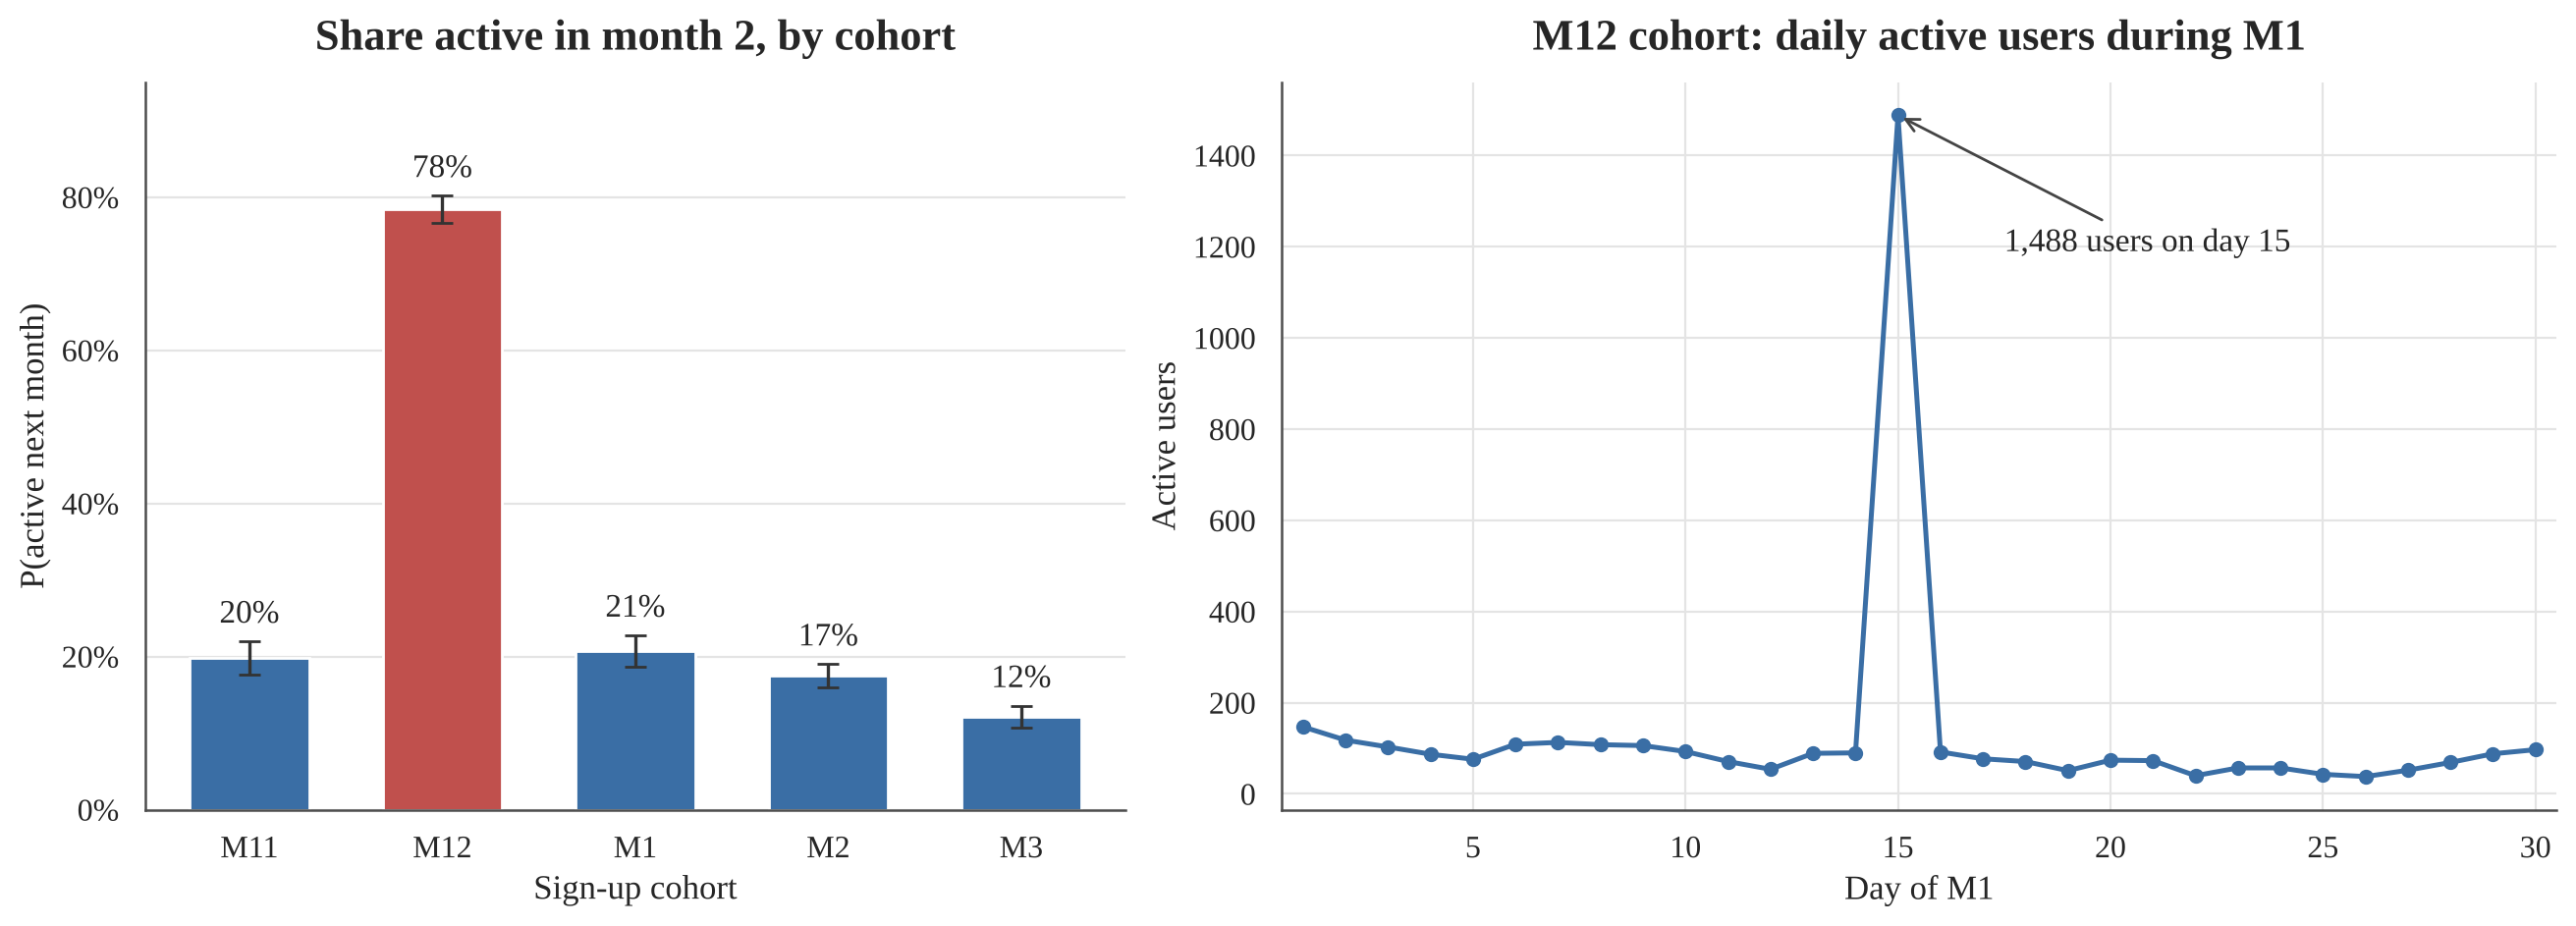
\includegraphics[width=0.95\linewidth]{fig03_cohorts}
\caption{Left: share active in month 2 per cohort (95\,\% CI). Right: daily active M12 users during M1.}
\label{fig:cohorts}
\end{figure}
Four of five cohorts retain 12--21\,\%, but \textbf{M12 retains 78\,\%} (Figure~\ref{fig:cohorts}). Its M1 activity is one spike of about 1\,500 users on day 15,
concentrated on competition \code{ID\_528W}, a secret-code hackathon. Most M12 sign-ups were event participants, and the event itself caused their ``retention''.
\begin{itemize}
  \item The label prior is not stationary, so a random split would mix cohorts and look over-optimistic $\Rightarrow$ \textbf{time-based validation}.
  \item M12 is not representative of the test cohort $\Rightarrow$ we test \textbf{excluding it from training}.
  \item This motivated the features \code{joined\_hackathon} and \code{n\_new\_comps\_joined}.
\end{itemize}

\subsection{First-month engagement}
\begin{figure}[H]\centering
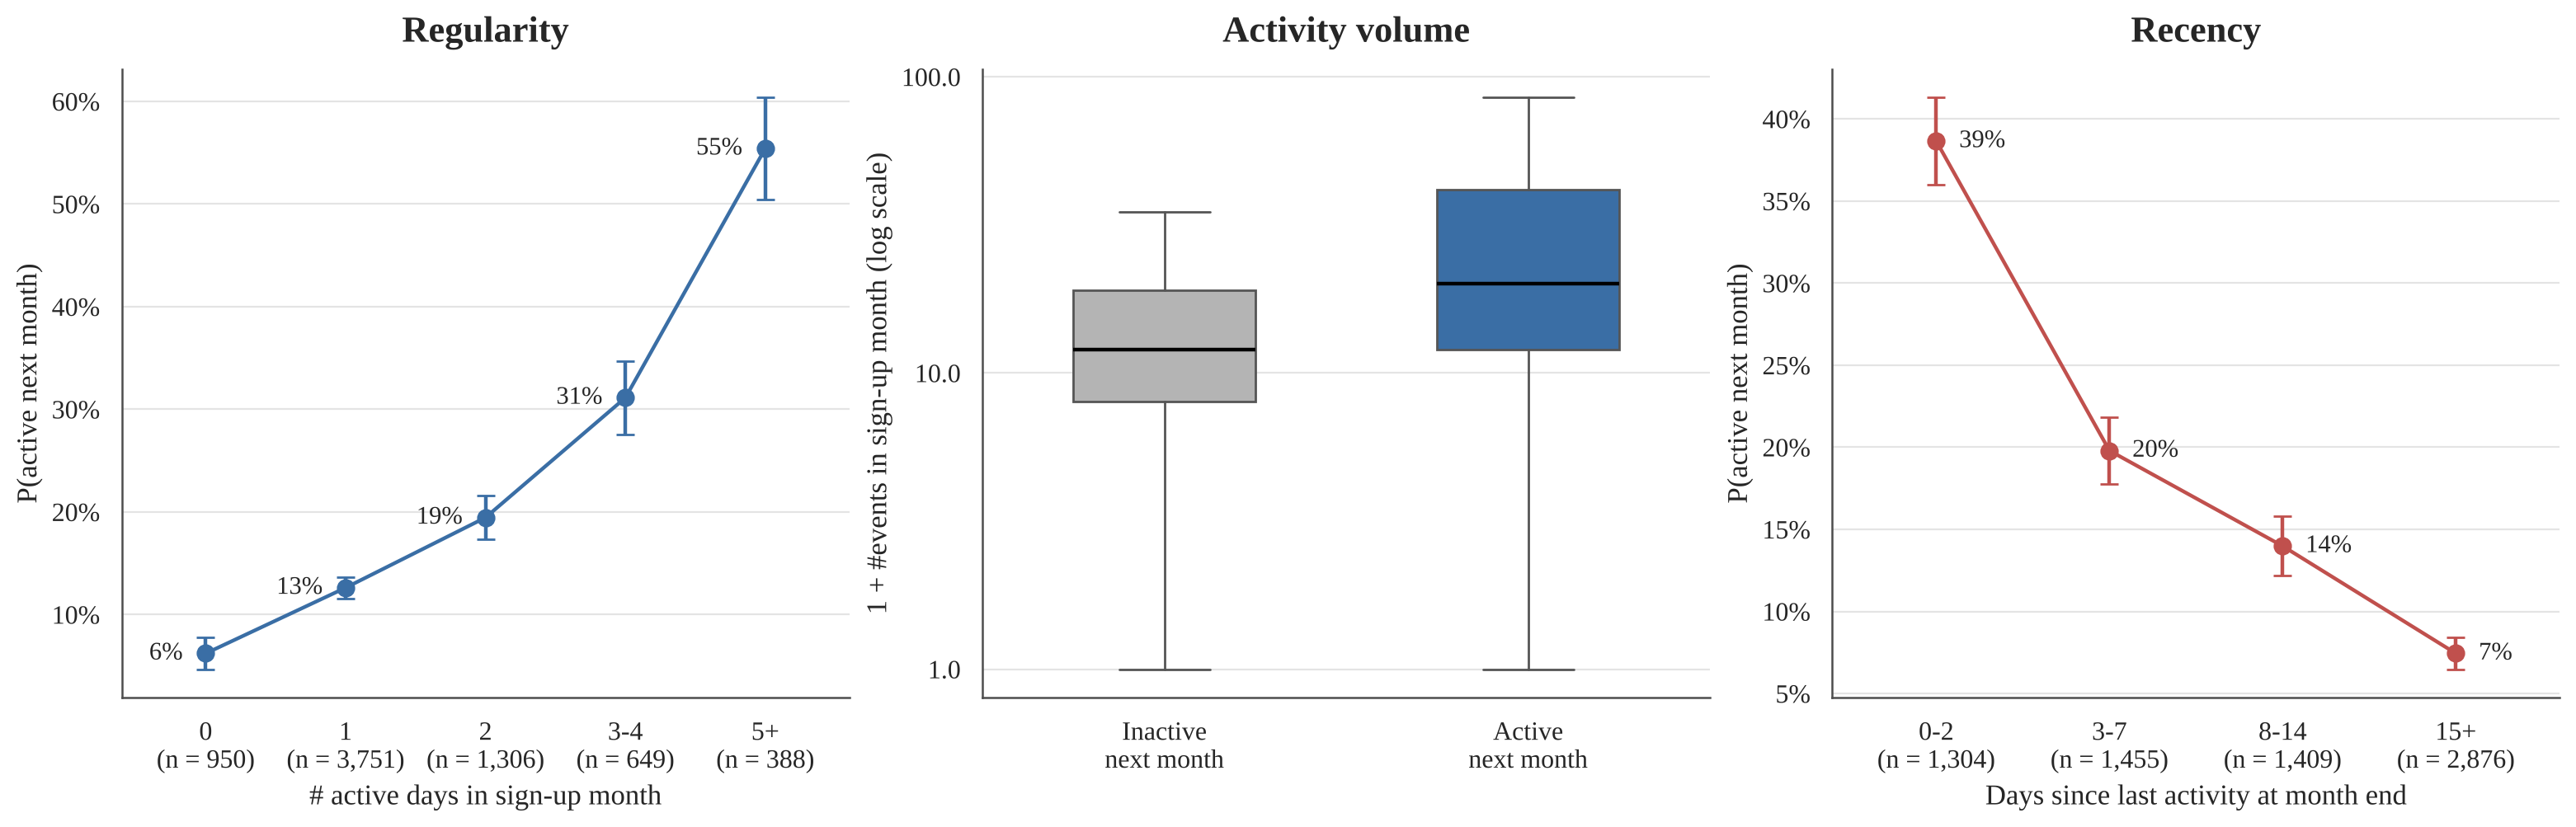
\includegraphics[width=\linewidth]{fig04_engagement}
\caption{Typical cohorts: retention by number of active days, event volume by outcome (log scale), retention by recency.}
\label{fig:eng}
\end{figure}
Retention rises monotonically with the number of active days, from 6\,\% (no logged activity) to 55\,\% (5+ days).
Recency matters at least as much: users seen in the last two days of the month return 39\,\% of the time, against 7\,\% for users silent for 15+ days.
The counts are very right-skewed $\Rightarrow$ log-transform them for the linear model (tree models are invariant to this).

\subsection{Behaviour types, profile variables and correlations}
\begin{figure}[H]\centering
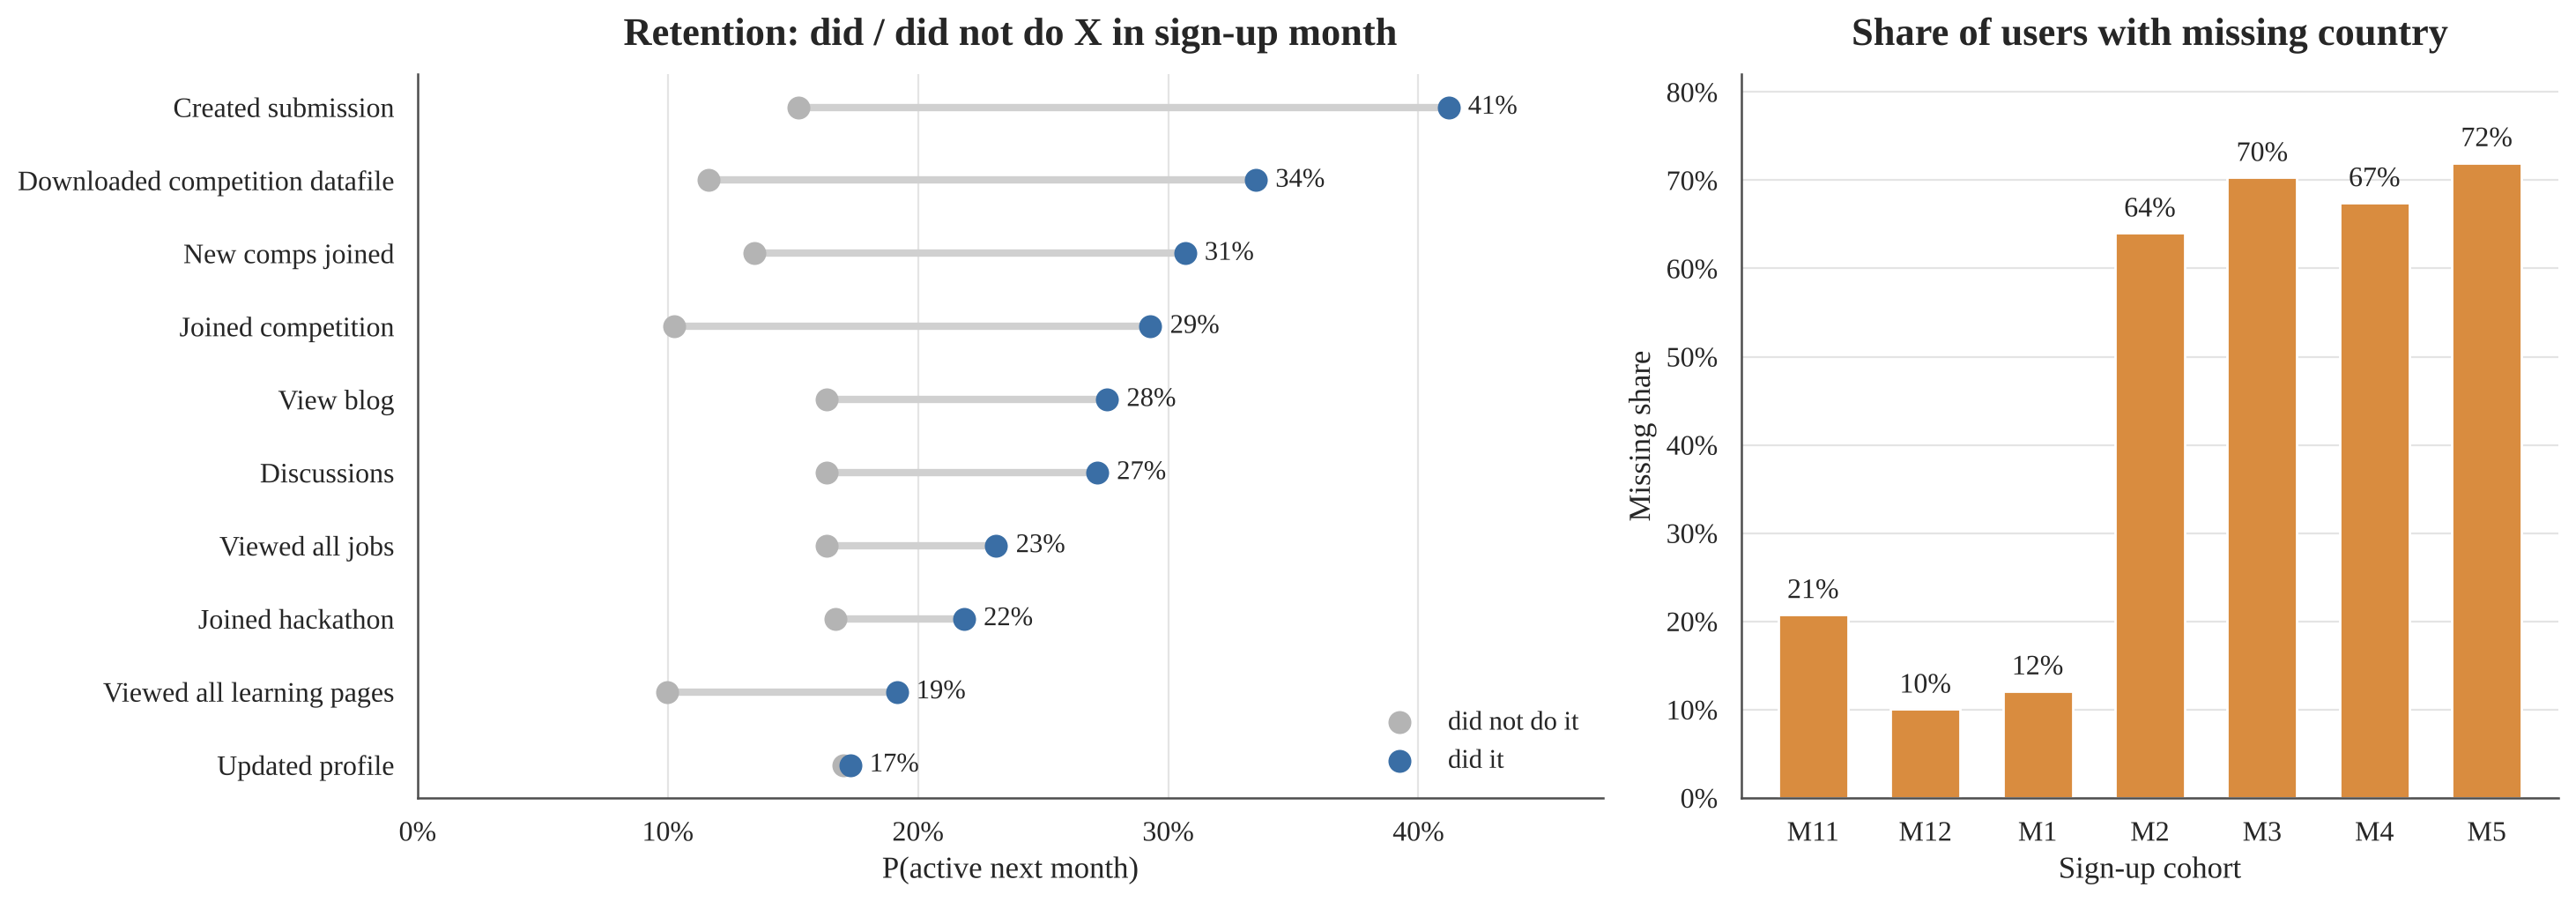
\includegraphics[width=\linewidth]{fig05_behaviour}
\caption{Left: retention of users who did or did not do each action. Right: share of users with missing country per cohort.}
\label{fig:beh}
\end{figure}
\emph{Doing} things (submitting, downloading data, joining competitions, posting) predicts retention much better than \emph{reading} blog or jobs pages
$\Rightarrow$ keep the behaviour-family breakdown. Country is missing for 10--21\,\% of users up to M1 and 64--72\,\% from M2 on,
which points to a change in the sign-up form. \code{country\_missing} is therefore a time proxy $\Rightarrow$ we test dropping the country features.
Activity features are strongly collinear (Spearman $\rho$ 0.6--0.9, Figure~\ref{fig:corr}) $\Rightarrow$ L2-regularised logistic regression; trees handle collinearity natively.

\begin{figure}[H]\centering
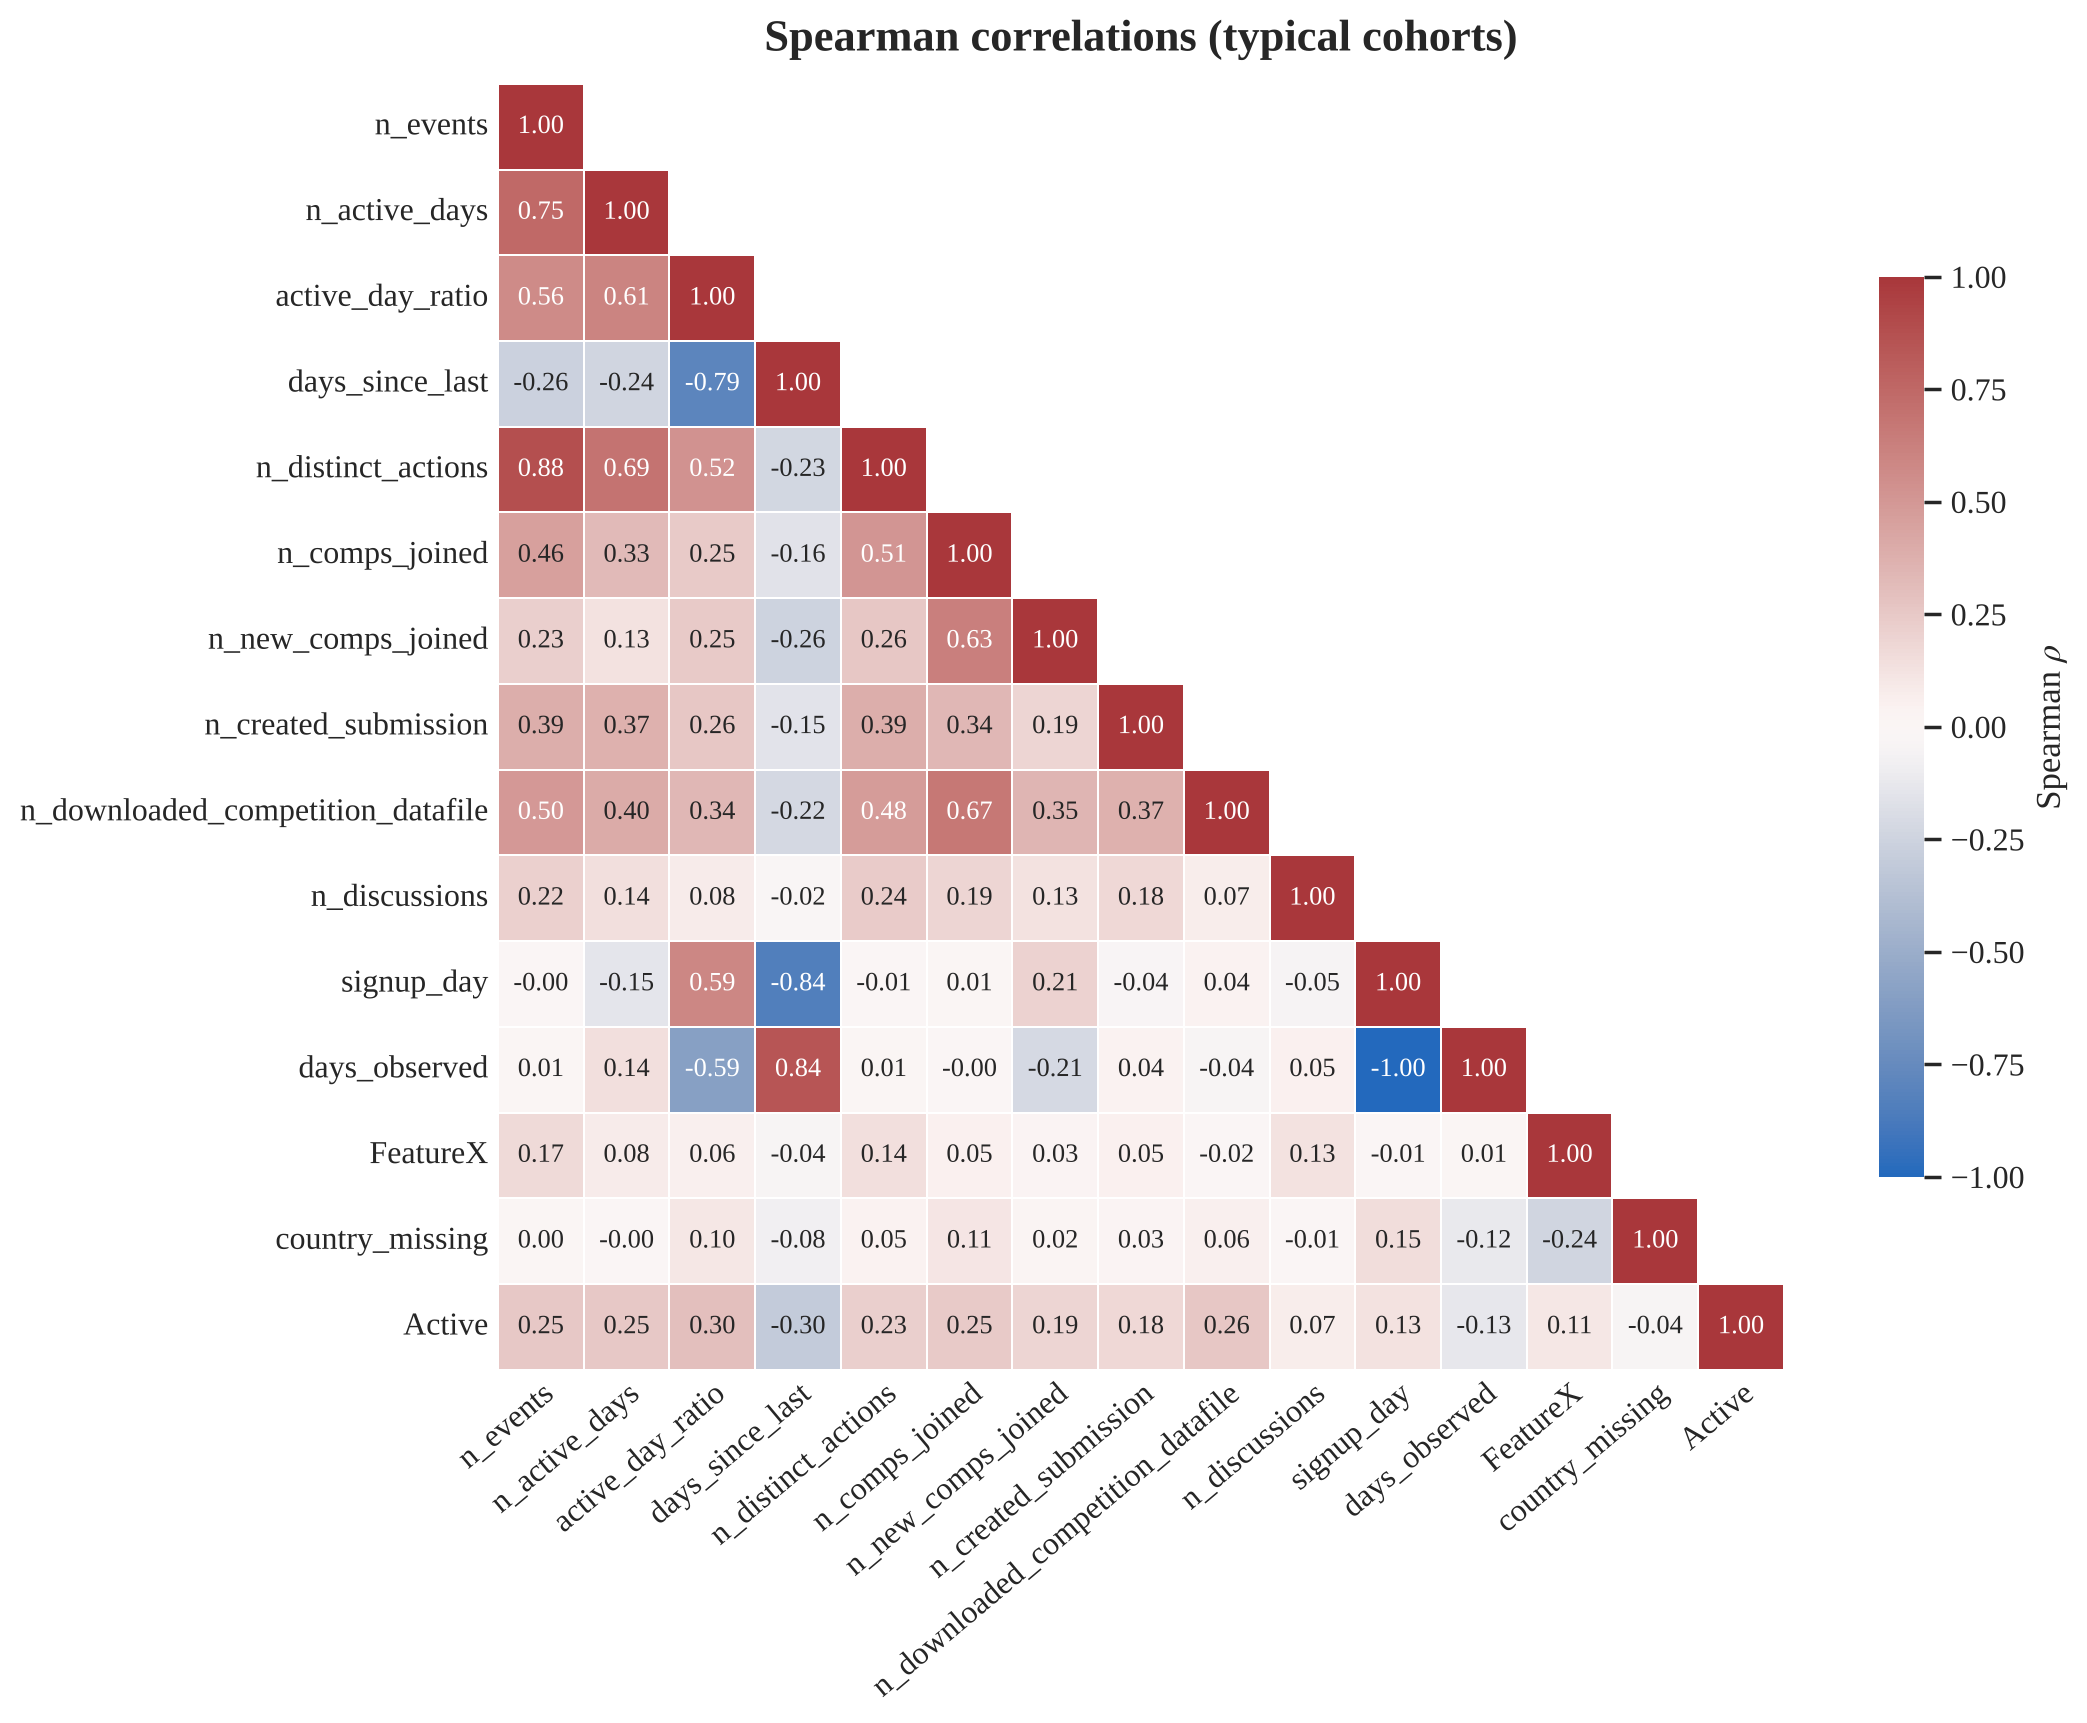
\includegraphics[width=0.6\linewidth]{fig06_correlation}
\caption{Spearman correlations (typical cohorts).}\label{fig:corr}
\end{figure}

%=====================================================================
\section{Validation design, metric and models}
\label{sec:val}

\subsection{Cross-validation: forward chaining by cohort}
At deployment the model is trained on past cohorts and applied to a new one, so validation must do the same:
\begin{table}[H]\centering\small
\begin{tabular}{lll}\toprule
Split & Train cohorts & Validate on\\\midrule
Inner fold 1 & M11 (+M12) & M1\\
Inner fold 2 & M11 (+M12), M1 & M2\\
\textbf{Hold-out test} & M11 (+M12), M1, M2 & \textbf{M3} (never used for tuning)\\\bottomrule
\end{tabular}
\end{table}
Hyper-parameters and the model family are chosen on the two inner folds. The decision threshold is chosen on the inner out-of-fold predictions,
and M3 is scored once at the end. Figure~\ref{fig:kfold} shows why random K-fold is wrong here: it reports PR-AUC 0.85,
while forward validation gives 0.30--0.47, because the model memorises cohort-specific signals that do not carry over to a future cohort.

\begin{figure}[H]\centering
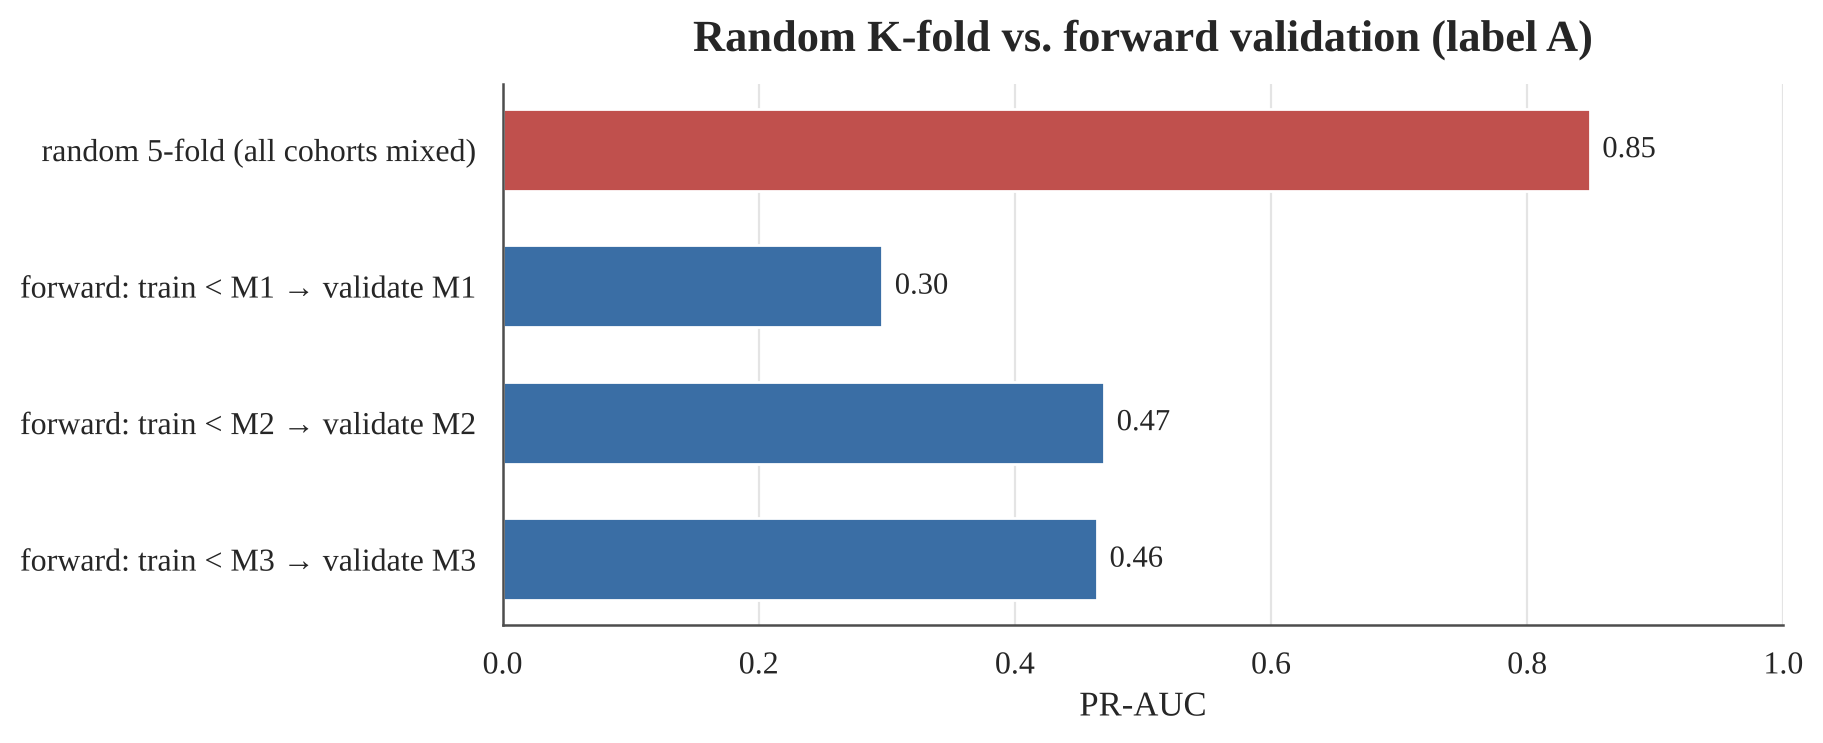
\includegraphics[width=0.62\linewidth]{fig07_kfold}
\caption{PR-AUC of a default gradient-boosting model under random 5-fold CV and under forward validation.}\label{fig:kfold}
\end{figure}

\subsection{Metric}
\textbf{F1 of the positive class} is the competition metric. Positives are only 12--21\,\% of a cohort, so accuracy is useless:
predicting ``all inactive'' gives 85\,\% accuracy and F1 = 0. F1 balances precision (do not waste the retention budget) and recall (do not miss engaged users).
For model selection we use the threshold-free \textbf{PR-AUC} (average precision), which focuses on the minority class.

\subsection{Models and hyper-parameter search}
\begin{itemize}
  \item \textbf{Rule-of-thumb baseline}, ``active on $\ge k$ days'', with $k$ tuned on the inner folds: what a product manager would do without ML.
  \item \textbf{Logistic regression} (log1p, scaling, L2, class-balanced): interpretable and robust to shift.
  \item \textbf{Random forest} (class-balanced): non-linear, few assumptions.
  \item \textbf{Histogram gradient boosting}: strong on tabular data, handles skewed counts and interactions.
\end{itemize}
\code{GridSearchCV} with our forward folds and PR-AUC scoring covers $C$ for logistic regression; depth, leaf size and \code{max\_features} for the forest;
and learning rate, iterations, leaf nodes, leaf size and L2 for boosting. Two data choices from the EDA are crossed with every grid:
keep or drop M12 in training, and keep or drop the country features. The whole procedure is run once for label A and once for label B.

\begin{table}[H]\centering\small
\begin{tabular}{llcccc}\toprule
& & \multicolumn{2}{c}{M12 dropped} & \multicolumn{2}{c}{M12 kept}\\\cmidrule(lr){3-4}\cmidrule(lr){5-6}
Label & Model & all features & no country & all features & no country\\\midrule
A & GradBoost & 0.499 & \textbf{0.508} & 0.425 & 0.425\\
A & RandomForest & 0.500 & 0.498 & 0.446 & 0.470\\
A & LogReg & 0.471 & 0.474 & 0.436 & 0.450\\\midrule
B & GradBoost & 0.491 & \textbf{0.495} & 0.398 & 0.392\\
B & RandomForest & 0.484 & 0.488 & 0.433 & 0.459\\
B & LogReg & 0.463 & 0.467 & 0.427 & 0.440\\\bottomrule
\end{tabular}
\caption{Best cross-validated PR-AUC per model and data choice.}\label{tab:cv}
\end{table}
Dropping M12 from training helps every model under both labels: the event-driven cohort teaches the wrong base rate.
The country features have a small and inconsistent effect. Both labels select \textbf{gradient boosting without M12 and without country}
(learning rate 0.03, 100 iterations, 7 leaf nodes, min.\ 80 samples per leaf).

%=====================================================================
\section{Results}
\label{sec:results}

\subsection{Hold-out cohort M3: label A vs.\ label B}
\begin{table}[H]\centering\small
\begin{tabular}{llcccccc}\toprule
Label & Model & Threshold & F1 & Precision & Recall & PR-AUC & ROC-AUC\\\midrule
A & \textbf{GradBoost (selected)} & 0.32 & \textbf{0.472} & 0.451 & 0.494 & 0.479 & 0.830\\
A & RandomForest & 0.60 & 0.462 & 0.412 & 0.527 & 0.451 & 0.817\\
A & LogReg & 0.61 & 0.484 & 0.433 & 0.547 & 0.482 & 0.820\\
A & Rule: active days $\ge 2$ & -- & 0.359 & 0.259 & 0.588 & -- & --\\
A & Everyone active & -- & 0.217 & 0.122 & 1.000 & 0.122 & 0.500\\\midrule
B & \textbf{GradBoost (selected)} & 0.32 & \textbf{0.450} & 0.440 & 0.460 & 0.466 & 0.829\\
B & RandomForest & 0.62 & 0.450 & 0.408 & 0.502 & 0.443 & 0.816\\
B & LogReg & 0.63 & 0.468 & 0.435 & 0.506 & 0.485 & 0.826\\
B & Rule: active days $\ge 3$ & -- & 0.396 & 0.383 & 0.410 & -- & --\\
B & Everyone active & -- & 0.213 & 0.120 & 1.000 & 0.120 & 0.500\\\bottomrule
\end{tabular}
\caption{Hold-out results on M3 (243 positives under A, 239 under B).}\label{tab:hold}
\end{table}

\begin{figure}[H]\centering
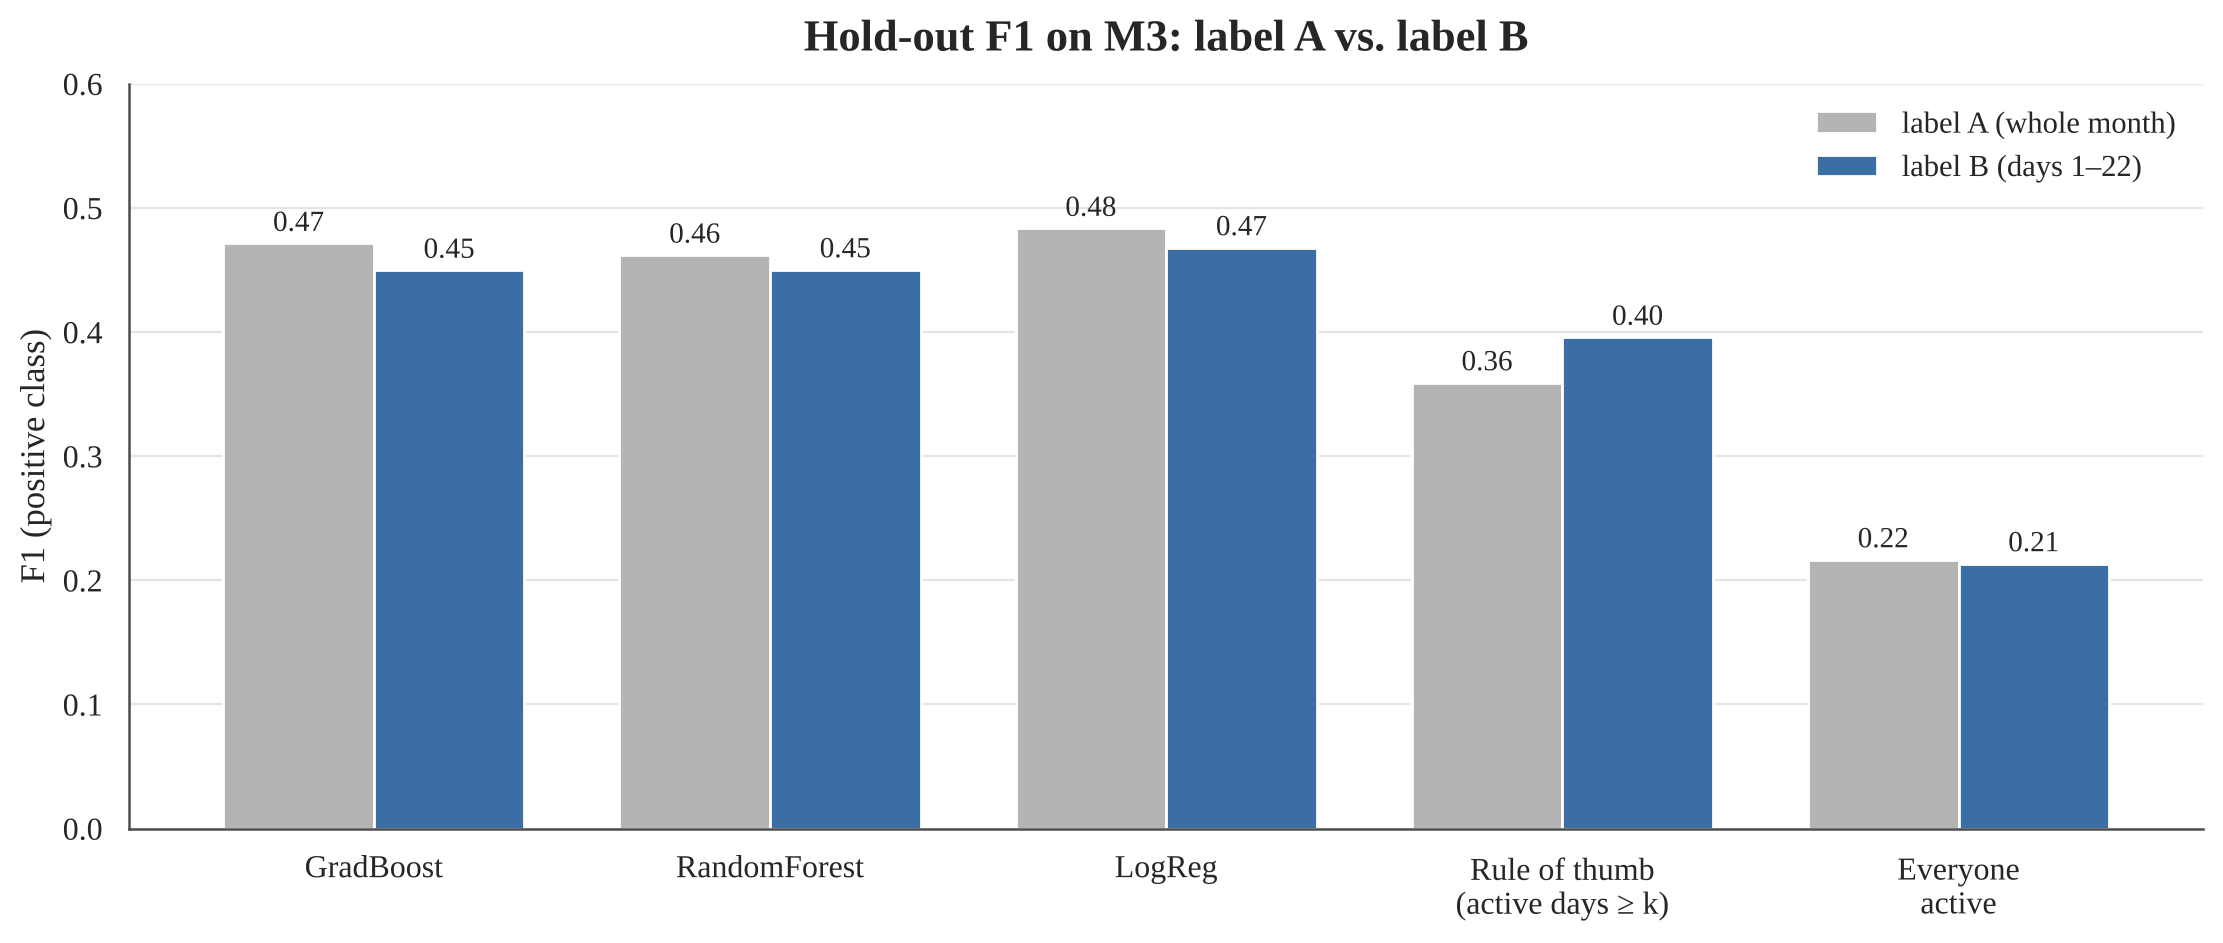
\includegraphics[width=0.8\linewidth]{fig09_compare}
\caption{Hold-out F1 on M3 for every model under both labels.}\label{fig:compare}
\end{figure}

\begin{figure}[H]\centering
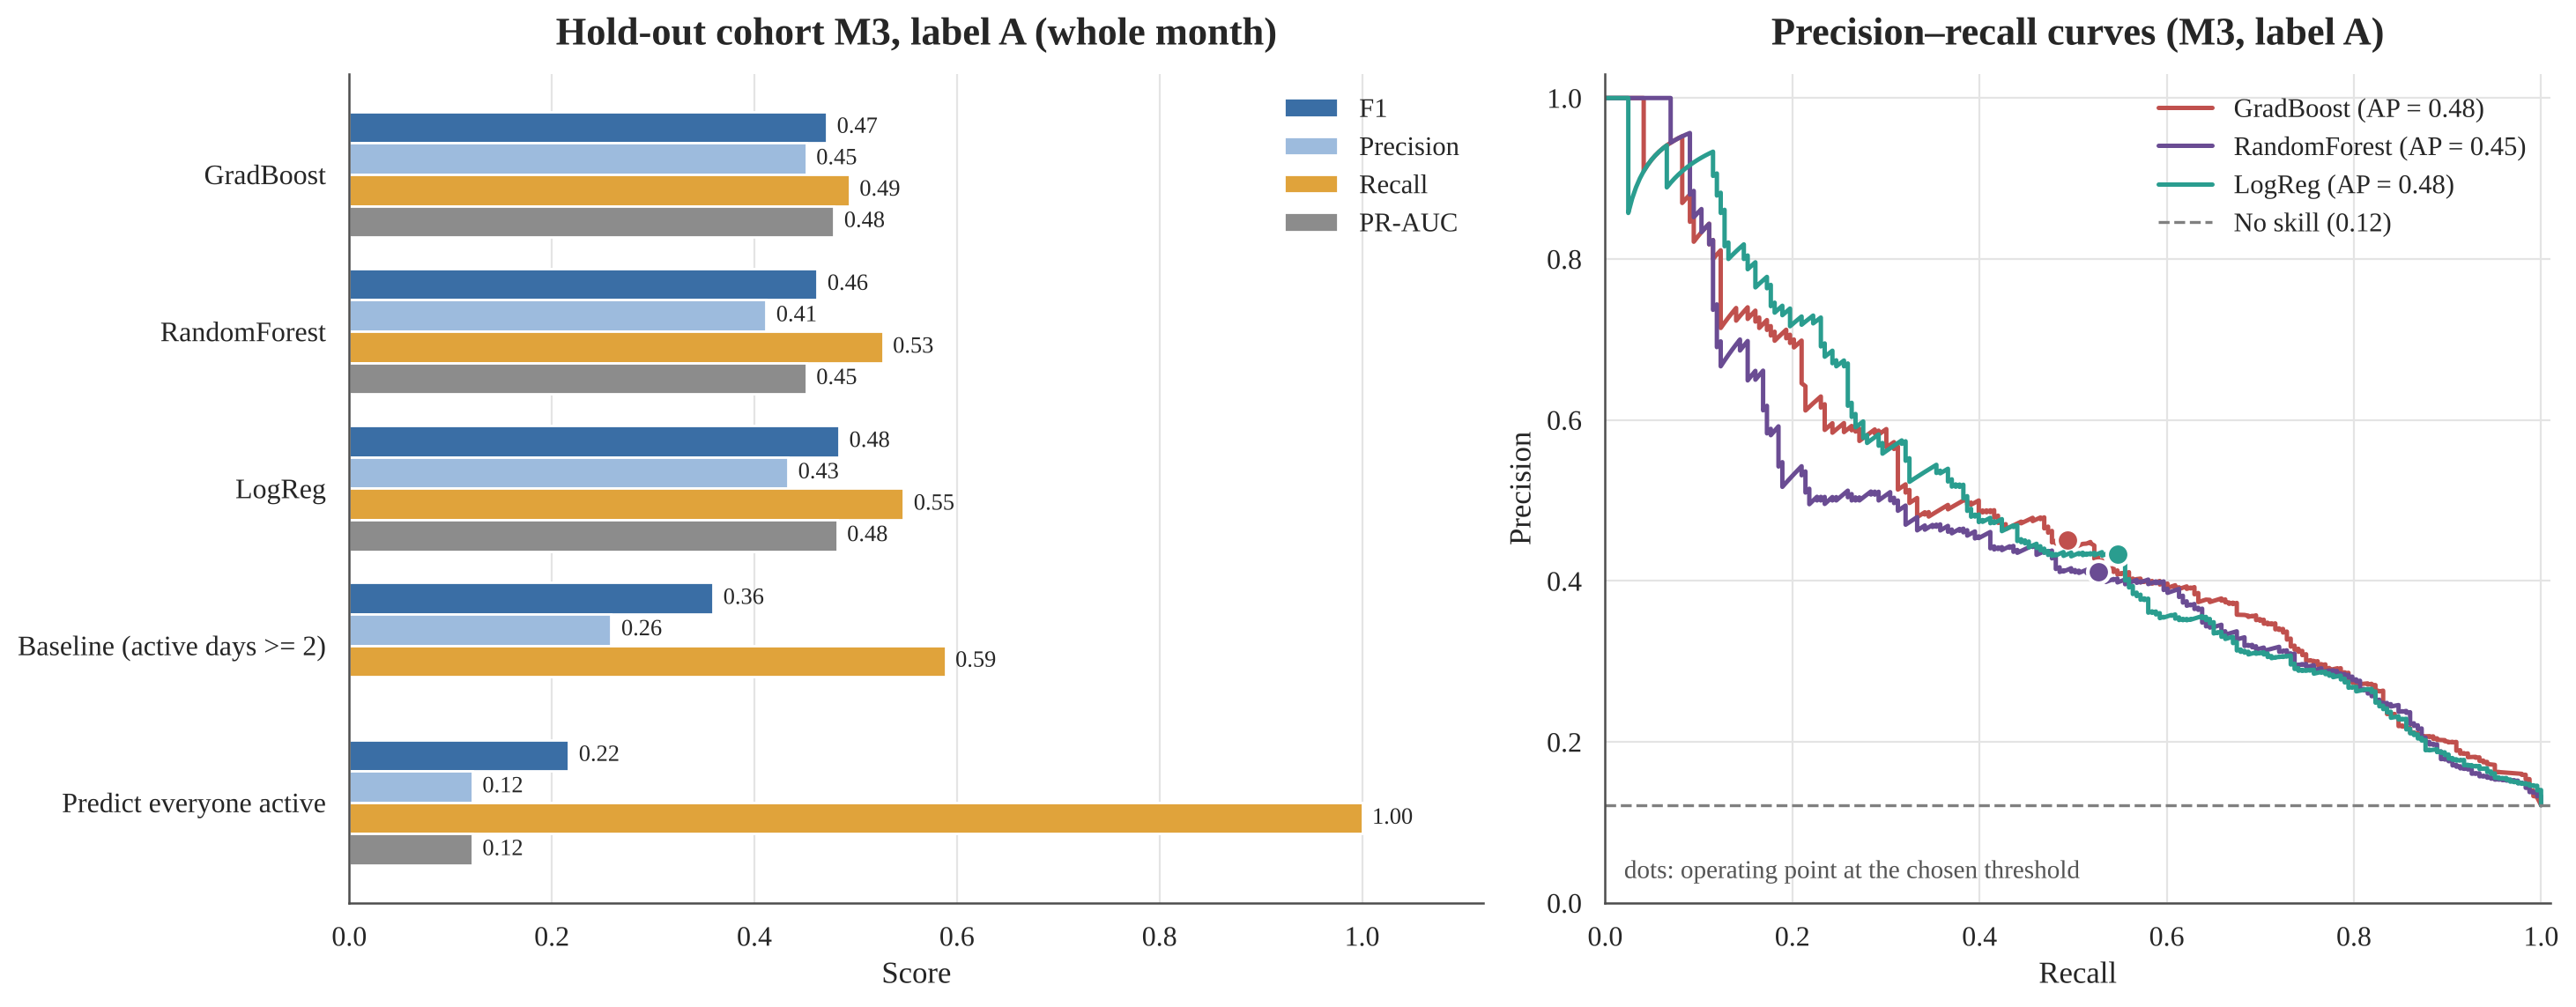
\includegraphics[width=\linewidth]{fig08_holdout_A}\\[4pt]
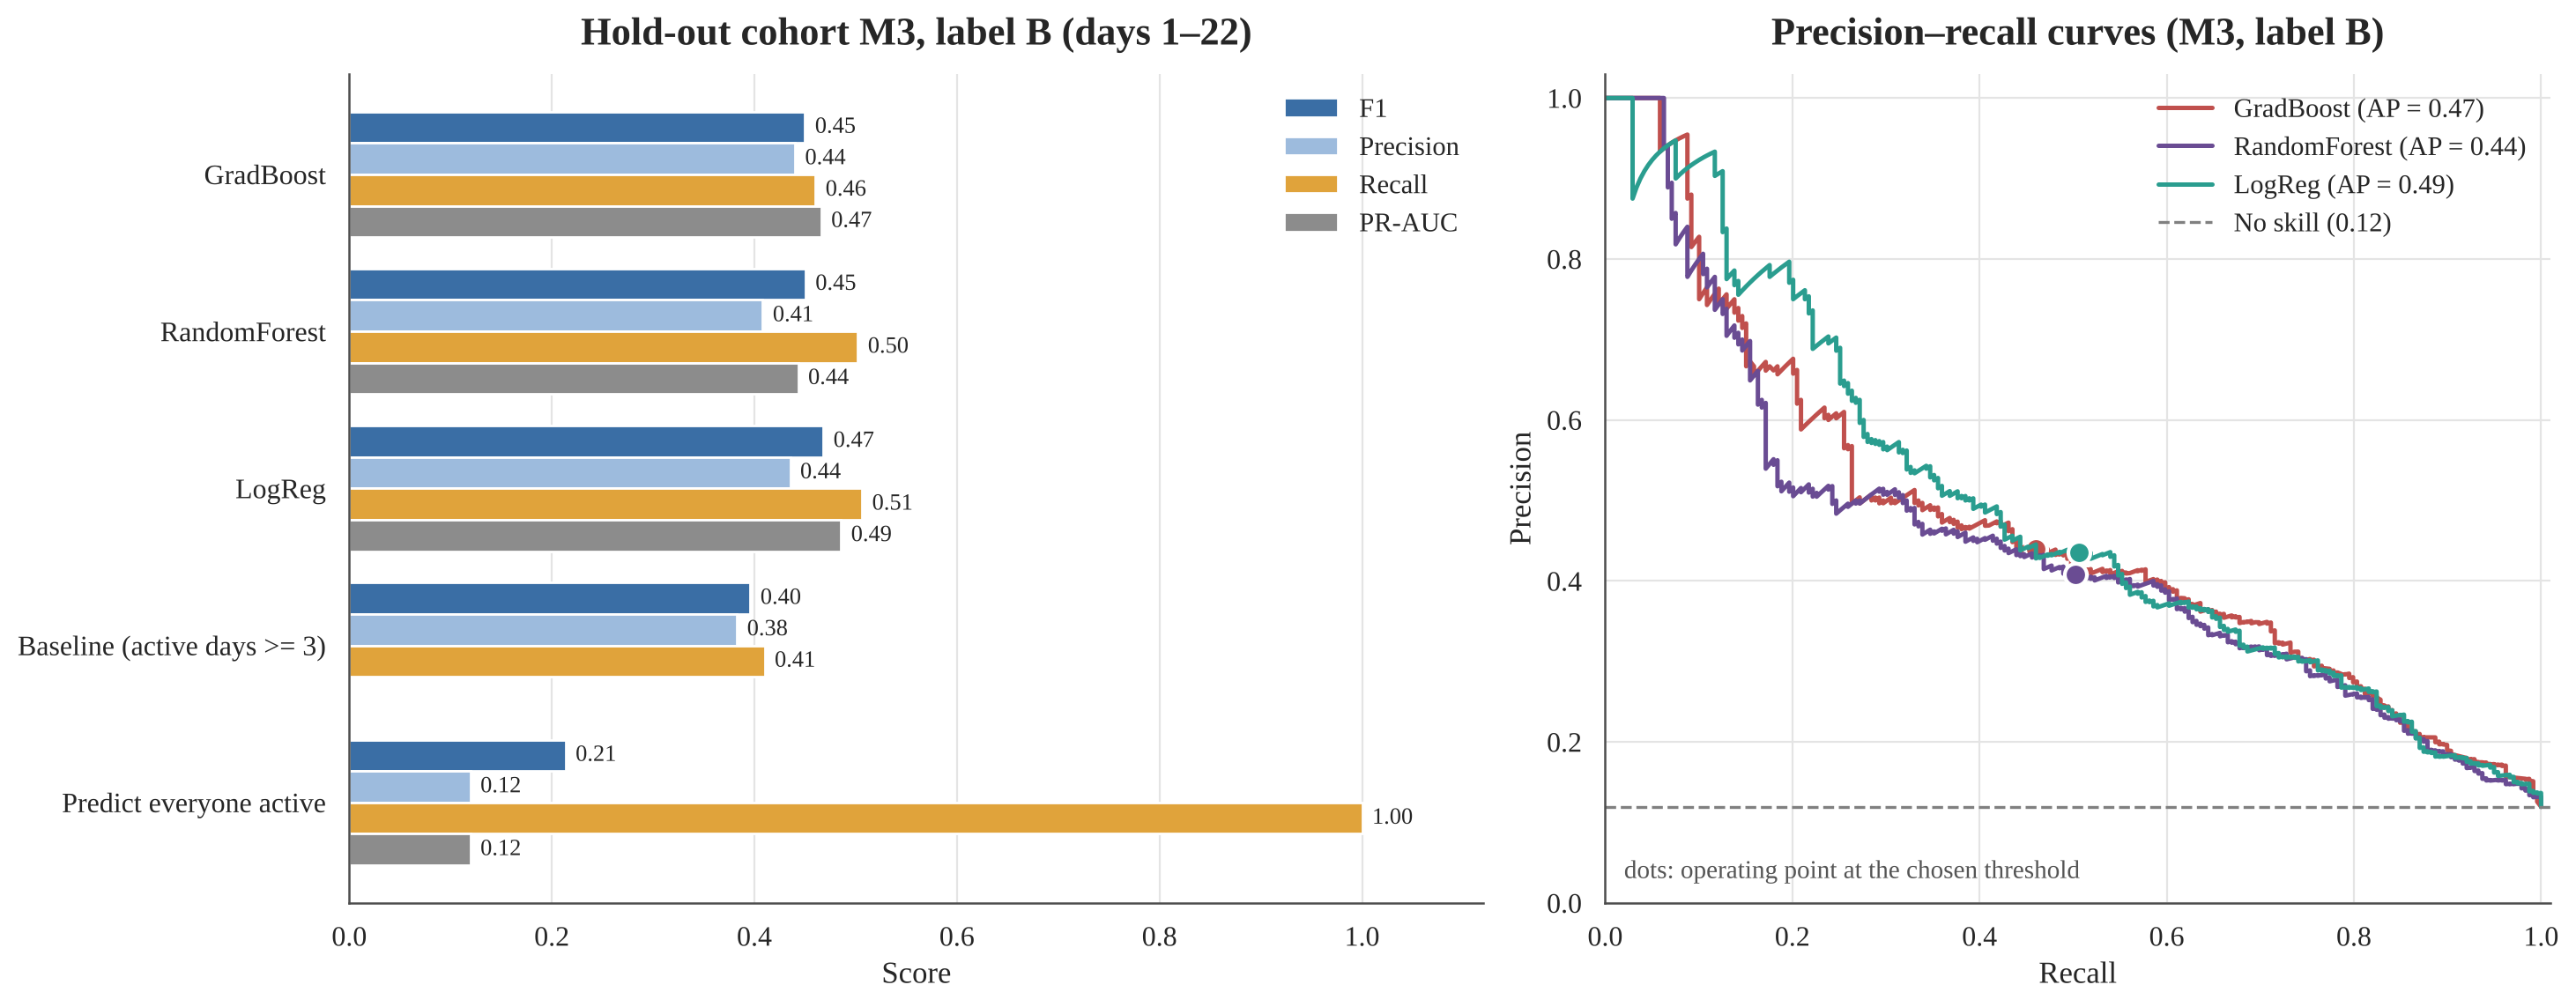
\includegraphics[width=\linewidth]{fig08_holdout_B}
\caption{Hold-out metrics and precision--recall curves, label A (top) and label B (bottom).}\label{fig:holdout}
\end{figure}

\begin{itemize}
  \item \textbf{Label A:} the selected model reaches F1 = 0.47 on M3. This number mixes two label definitions: the training labels count late returners, but the M3 labels almost cannot.
  \item \textbf{Label B:} F1 = \textbf{0.45}. Training and test labels are measured the same way, so this is the \textbf{consistent estimate} for a future cohort.
  \item The difference (about 0.02 F1) is within the noise of a $\sim$240-positive cohort. The model choice and the conclusions are the same, so the original result was not badly wrong, but only label B is methodologically clean.
  \item The three ML models are within $\sim$0.02 F1 of each other. We keep the CV-selected model rather than picking on the hold-out.
  \item Every ML model beats the rule of thumb (+0.05 to +0.12 F1) and ``everyone active'' (+0.24 F1 or more).
\end{itemize}

\subsection{What drives the model?}
\begin{figure}[H]\centering
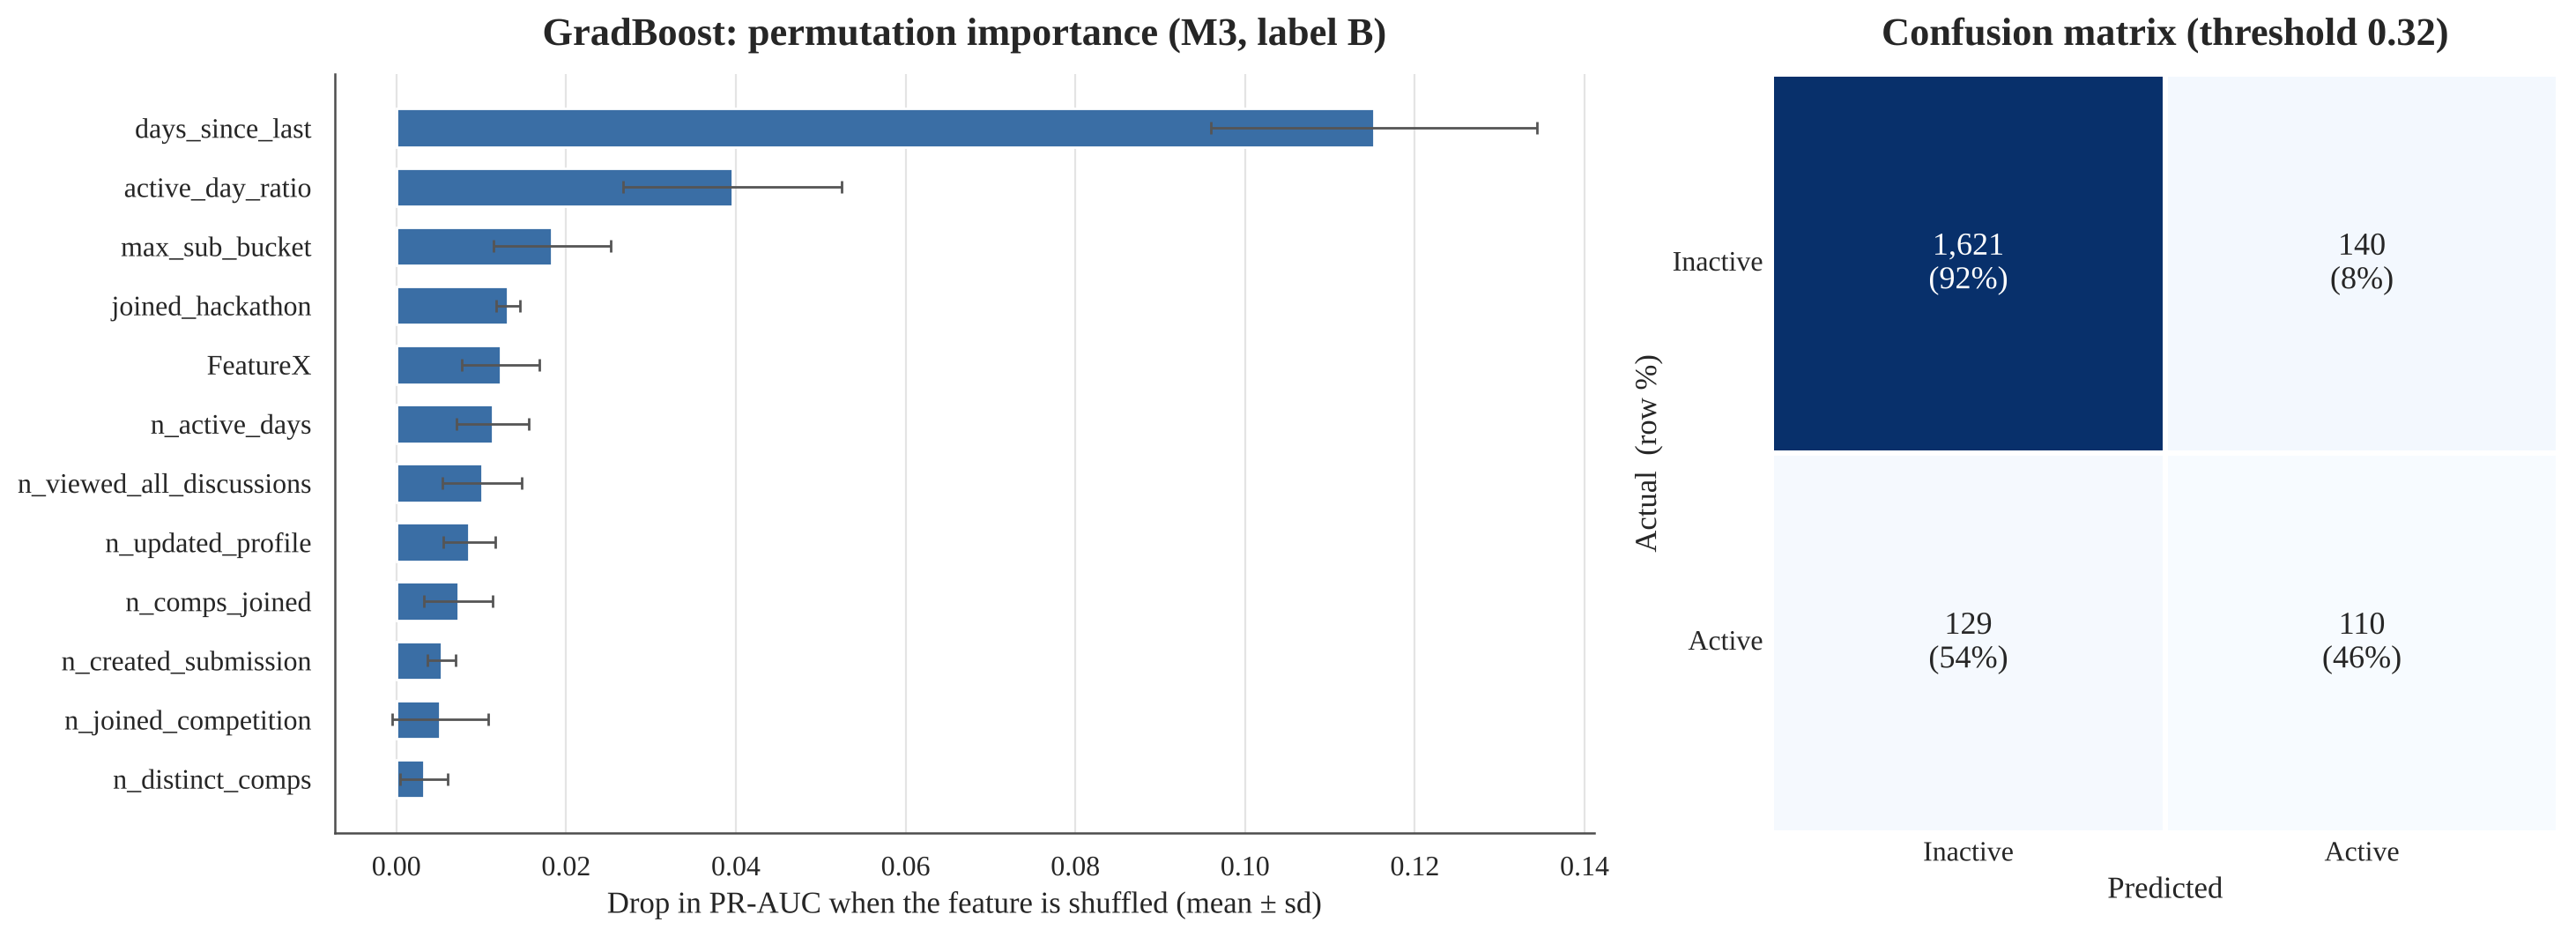
\includegraphics[width=\linewidth]{fig10_drivers_B}
\caption{Permutation importance on M3 and confusion matrix at the chosen threshold (label B; label A gives the same top features).}\label{fig:drivers}
\end{figure}
{\sloppy Recency (\code{days\_since\_last}) is by far the strongest signal.
Regularity (\code{active\_day\_ratio}, \code{n\_active\_days}) and \emph{doing} signals
(successful-submission bucket, hackathon, competitions joined, submissions) come next. Profile variables add little, and country was dropped by the search:
engagement is about behaviour, not demographics, which is good for fairness and for acting on the predictions.
At the chosen threshold the label-B model finds 46\,\% of returners with 44\,\% precision, about 3.7 times the 12\,\% base rate. \par}

%=====================================================================
\section{Real-world impact}
\label{sec:impact}
\begin{figure}[H]\centering
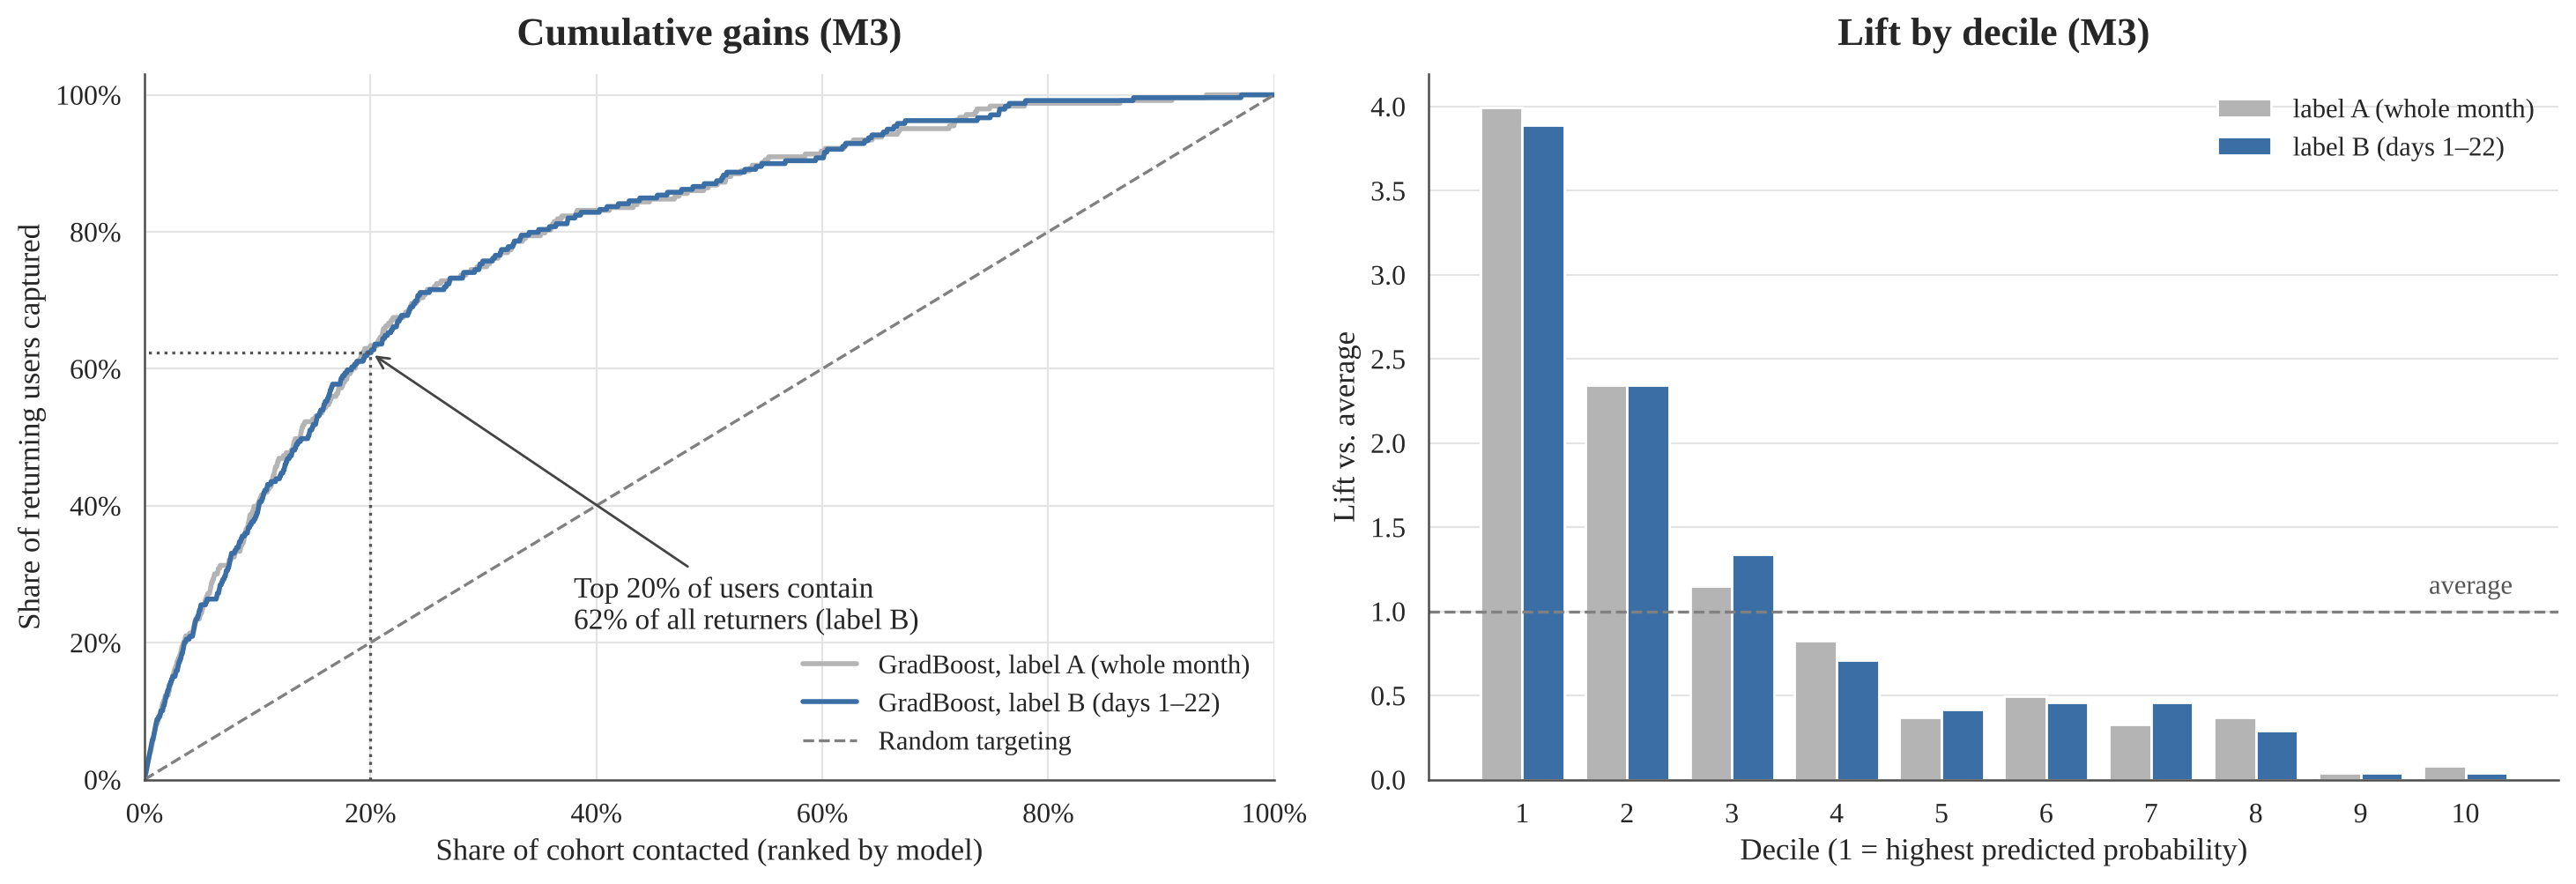
\includegraphics[width=\linewidth]{fig11_gains}
\caption{Cumulative gains and lift by decile on M3 for the selected model under both labels.}\label{fig:gains}
\end{figure}
A retention campaign has a budget, so it contacts the top $x$\,\% of users ranked by the model. The two labels give almost the same curves (Figure~\ref{fig:gains}):
\begin{itemize}
  \item The \textbf{top 20\,\%} of users by score contain \textbf{62\,\%} (B) / 63\,\% (A) of all returners; the bottom half contains only 13\,\%.
  \item The \textbf{top decile} is about \textbf{4$\times$} more likely to return than average, which makes it the natural shortlist for hackathon invitations and ambassador programmes.
  \item \textbf{Illustrative business case} (our assumptions): with 2\,000 sign-ups per month and an intervention costing 5 USD per user, contacting everybody costs 10\,000 USD.
        Contacting only the 40\,\% ``uncertain'' middle segment costs 4\,000 USD (\textbf{$-$60\,\%}) and still covers the users whose behaviour can plausibly be changed.
  \item The \emph{causal} effect of an intervention cannot be estimated from observational data, so an \textbf{A/B test} is needed before claiming revenue impact.
\end{itemize}

\paragraph{Official test cohort (M4).} Each label's model is refit on all labelled cohorts (without M12) with its own threshold.
\code{submission\_label\_A.csv} predicts ``active at any time in M5'' (the competition's target, 10.9\,\% predicted active);
\code{submission\_label\_B.csv} predicts ``active in days 1--22 of M5'' (10.2\,\%). Both rates are plausible given the 12\,\% base rate.

%=====================================================================
\section{Conclusions}
\label{sec:conclusion}
\paragraph{Findings.}
\begin{itemize}
  \item The labelled training set had to be reconstructed: we recovered the month order from the data and built the target. The latest labelled cohort, M3, is the hold-out.
  \item The truncated M4 log creates a label-definition inconsistency between training and test. Measuring every cohort over days 1--22 removes it at a cost of about 0.02 F1.
  \item Recency and regularity of first-month activity predict month-2 retention far better than demographics; doing beats browsing.
  \item Retention is non-stationary: one hackathon raised a cohort's retention to 78\,\%, and a form change made country missing for most later users.
\end{itemize}

\paragraph{Remarks on the ML experiments.}
Random K-fold would have overstated performance about 2$\times$. Excluding the event-driven cohort was the most useful data decision,
and validation design mattered more than the model family. Limits: only five labelled cohorts (noisy fold estimates), masked features,
label B ignores returns after day 22 (about 10\,\% of returners), and event cohorts depend on an external competition calendar.

\paragraph{Does the model solve the problem?}
Largely for \emph{ranking}, partly for \emph{exact classification}. On an unseen future cohort it reaches F1 = 0.45 with consistent labels
(0.47 with the original labels), compared with 0.36--0.40 for the best rule of thumb, and it puts 62\,\% of returners in the top 20\,\% of users.
That is enough to make targeted retention several times cheaper than a blanket campaign.
Absolute F1 stays moderate because many returns are triggered by future events (new competitions, hackathons) that cannot be seen in month 1.

\paragraph{Next steps.} Add the competition calendar (upcoming launches) as features, train on more cohorts,
calibrate probabilities per cohort, and measure business impact with an A/B-tested retention campaign.

\vspace{6pt}\noindent\small\textbf{Reproducibility.} All numbers and figures come from \code{notebook/zindi\_engagement.ipynb} (random seed 42).
\end{document}
